
\PassOptionsToClass{10pt}{article}
\documentclass{mcmthesis}
\usepackage{amsmath, amssymb, amsfonts} % 基础数学包
 \usepackage{dsfont}                      
 \usepackage{graphicx}                   % 支持图片插入
 \usepackage{booktabs}                   % 支持三线表 
 \usepackage{float}         
 \usepackage[font=small,labelfont=bf]{caption}
\usepackage{microtype}
\emergencystretch=2em

% ---- global space tightening (safe, content-neutral) ----
\setlength{\textfloatsep}{6pt plus 2pt minus 2pt}
\setlength{\floatsep}{6pt plus 2pt minus 2pt}
\setlength{\intextsep}{6pt plus 2pt minus 2pt}
\setlength{\abovecaptionskip}{2pt}
\setlength{\belowcaptionskip}{0pt}
\setlength{\abovedisplayskip}{6pt}
\setlength{\belowdisplayskip}{6pt}

\usepackage{enumitem}
\setlist{nosep,leftmargin=*}

\usepackage[font=small,labelfont=bf]{caption}
\captionsetup{skip=2pt}

\usepackage{titlesec}
\titlespacing*{\section}{0pt}{0.8ex}{0.4ex}
\titlespacing*{\subsection}{0pt}{0.6ex}{0.3ex}


 % 支持图片位置固定 [H]
 \usepackage[section]{placeins} % prevent floats crossing section boundaries
\usepackage{tocloft}

% =======================================================
% 【最终修正版】目录样式设置 (保留三级标题)
% =======================================================
% 1. 让目录标题 (Contents) 居中
\renewcommand{\cfttoctitlefont}{\hfill\Large\bfseries}
\renewcommand{\cftaftertoctitle}{\hfill}

% 2. 让一级标题 (Section) 强制显示引导点
\renewcommand{\cftsecleader}{\cftdotfill{\cftdotsep}}

% 3. 【关键修复】压缩行间距
% 减小目录标题下方距离
\setlength{\cftaftertoctitleskip}{5pt} 

% 减小一级标题 (Section) 之前的垂直距离


% 减小二级标题 (Subsection) 之前的垂直距离 (紧挨着)
\setlength{\cftbeforesubsecskip}{0pt}

% 减小三级标题 (Subsubsection) 之前的垂直距离 (紧挨着)
\setlength{\cftbeforesubsubsecskip}{0pt}

% 4. 控制目录深度 (改为 3，即显示到 4.1.1)
\setcounter{tocdepth}{3}
% =======================================================

% 3. (可选) 如果还不行，请取消下面这行的注释，强制设定点间距为 1
% \renewcommand{\cftsecdotsep}{1} 
% =======================================================


\usepackage{graphicx}
\usepackage{subcaption}
\graphicspath{{./}{./figures/}{./figure/}{./fig/}{./img/}{./image/}{./picture/}}
% --- 请将此段代码放入 main.tex 的导言区 (usepackage 之后) ---
\usepackage{amsthm} % 数学定理包
\theoremstyle{definition} % 设置样式
\newtheorem{definition}{Definition} % 定义 "Definition" 环境
\newtheorem{theorem}{Theorem}       % 定义 "Theorem" 环境
\newtheorem{axiom}{Assumption}      % 定义 "Assumption" 环境
% -----------------------------------------------------------
 % 当使用 CTeX 套装时请注释上一行使用该行的设置
\mcmsetup{tstyle=\color{red}\bfseries,%修改题号，队号的颜色和加粗显示，黑色可以修改为 black
tcn = 2619541, problem =C, %修改队号，参赛题号
sheet = true, titleinsheet = true, keywordsinsheet = true,
titlepage = false, abstract = true}
\usepackage{float}
%四款字体可以选择
\usepackage{times}
%\usepackage{newtxtext}
%\usepackage{palatino}
%\usepackage{txfonts}

\usepackage[utf8]{inputenc}
\usepackage{indentfirst}  %首行缩进，注释掉，首行就不再缩进。
\usepackage{lipsum}

%\usepackage{ctex}

\title{PAGS: Auditing DWTS Voting Aggregation Rules via Inverse Reconstruction and Counterfactual Simulation}
















\begin{document}
\setlength{\cftaftertoctitleskip}{5pt}
\setlength{\cftbeforesecskip}{5pt}
\setlength{\cftbeforesubsecskip}{2pt}


\begin{abstract}
Persistent controversy in televised dance competitions reflects a structural tension between judges’ technical evaluations and audience voting: strong performers may exit under transient vote swings, whereas popularity-dominant contestants can become effectively “locked in,” eroding perceived competitive legitimacy. Because vote totals are unobserved, audience support must be inferred before the institutional effects of rule design can be audited.

For Problem 1, we propose an \textbf{inverse reconstruction framework} that models weekly audience support as a simplex-valued share vector and samples the rule-feasible region jointly implied by published procedures and observed eliminations. Operable weeks are screened by a feasibility-based diagnostic, and the reconstructed latent votes are validated on elimination weeks with a binary-outcome Posterior Predictive Consistency (PPC) of $90.5\%$.

For Problem 2, a \textbf{same-week counterfactual design} fixes each week’s realized information and varies only the voting aggregation rule. Rank aggregation stabilizes outcomes by buffering score--vote gaps yet can obscure substantive technical separation; percent aggregation preserves intensity of support and better reflects audience intent but magnifies the risk of extreme popularity. Counterfactual simulations show that voting aggregation rules change the eliminated contestant in $26\%$ of historical weeks. Judge-save layers can mitigate anomalous weeks, but opaque activation invites perceptions of discretionary interference.

For Problem 3, a \textbf{three-channel structure} couples judges’ scores, conditional audience preference, and an explicit survival-risk channel via discrete-time hazard modeling, enabling professional-partner contributions to be decomposed into technical uplift and popularity spillover and translated into changes in elimination hazard.

For Problem 4, PAGS (Professional--Adaptive Guard System) replaces discretionary intervention with rule-based safeguards through adaptive vote compression, phase-dependent weighting to strengthen late-stage technical credibility, and a minimal-intervention guardrail triggered only by statistically intolerable technical collapse. Historical simulations indicate that \textbf{the professionalism index (P, measuring alignment with technical scoring) increases from $0.419$ to $0.497$}. In the Bobby Bones stress test, PAGS re-calibrates a near-lock-in baseline to an $85.6\%$ elimination probability, aligning survival likelihood more closely with technical merit. Robustness is supported by sampling convergence, prior perturbations with negligible drift in key signals, and cross-model agreement of driver rankings. Findings are distilled into a producer-facing memo to guide transparent evaluation and revision of future rules.
\end{abstract}

\begin{keywords}
bayesian inverse reconstruction; counterfactual simulation; discrete-time hazard model; voting aggregation rules; PAGS architecture; agency--meritocracy trade-off.
\end{keywords}


\maketitle
%\setcounter{tocdepth}{2} % 只显示到二级标题 (Section 和 Subsection)，隐藏三级细节
%\tableofcontents
\tableofcontents
%\setlength{\cftparskip}{10pt}    % 目录项内部的行间距，0pt为紧凑，可改5pt/10pt
\setlength{\cftbeforesecskip}{3pt} % 一级标题（章节）之间的垂直间距，按需调整
%\tableofcontents

\newpage
\section{Introduction}

\subsection{Problem Background}

Televised competitions that integrate expert judging with audience participation function as hybrid decision systems in which heterogeneous signals are aggregated into eliminations and final standings. Because these signals reflect different criteria and incentives, the aggregation rule itself becomes a consequential component of governance, shaping perceived legitimacy and competitive incentives alongside entertainment outcomes.

A key practical constraint is partial observability. Although weekly judge scores and eliminations are typically available, audience support is often unreported and can vary in intensity between weeks and seasons. This limits direct attribution of surprising outcomes to true audience preference versus structural effects induced by the scoring rule, and it complicates producer-facing explanations of fairness.

Long-running programs further exhibit regime heterogeneity: scoring procedures may change across eras, expert panels may vary in size, and limited expert interventions may be introduced to moderate extreme outcomes. These features make cross-season comparison nontrivial and require attention to how rule changes interact with uncertainty and exceptional cases.

In this context, the evaluation of alternative aggregation principles is operationally relevant. Percentage-based aggregation can preserve magnitude differences and thus amplify outlier advantages, whereas ordinal ranking can compress margins and reweight influence toward relative position. Therefore, a credible assessment hinges on understanding how rule design affects technical alignment, audience agency, and the stability of eliminations under uncertainty, particularly in highly contested weeks.

\subsection{Restatement of the Problem}

This paper examines how a competition that combines expert judging and audience participation converts heterogeneous evaluations into eliminations and season outcomes and how alternative rules may change those outcomes across seasons.

Problem One seeks to infer plausible weekly patterns of audience support that are not directly observed but are compatible with the recorded elimination history. It also requires characterizing the uncertainty of these inferences and assessing how consistently they align with the observed outcomes.

Problem Two asks how different aggregation rules for judges’ assessments and audience support would affect eliminations and final placements. The task is to compare the rule regimes across seasons, evaluate whether either regime systematically increases the influence of fan preference, and examine the outcomes in high-disagreement cases. It further requires assessing how an additional judge-intervention step applied to a low-performing subset would alter results and concluding with a forward-looking recommendation on the preferred rule structure.

Problem Three investigates how professional partners and celebrity attributes relate to competitive success and whether their associations differ between expert evaluations and audience support.

Problem Four requires proposing an alternative scoring-and-elimination system that better satisfies explicit performance objectives for the show, with justification grounded in historical behavior.

Problem Five requires synthesizing the findings into a concise producer-facing memo that provides actionable guidance consistent with the technical analysis.


\subsection{Our Work}



Our main goals are to address these issues that need to be explored: (\textbf{1}) infer latent week-level fan support consistent with observed eliminations and carry uncertainty forward via posterior diagnostics; (\textbf{2}) compare percentage- and rank-based rules through uncertainty-propagated counterfactual simulations, including regime-stratified summaries, volatility measures, and high-variance case stress tests with and without judge intervention; (\textbf{3}) separate expert scoring, conditional audience preference, and elimination risk to attribute outcome associations to professional partners and celebrity characteristics; (\textbf{4}) design and evaluate an alternative rule that improves merit alignment while preserving audience agency under historical simulation; (\textbf{5}) distill results into actionable recommendations for future seasons.


%-----------模型假设-------------------%
\section{Assumptions and Notations}

\textbf{Asm.1 (Closed weekly risk set).}
In each competition week, the set of active contestants is correctly identified from the records and the elimination outcomes are determined only among the contestants who are active in that week.

\textbf{Asm.2 (Comparable judge scoring within a week).}
Within the same week, judges’ scores are on a common scale after aggregation and standardization, and missing judge entries represent judge absence rather than zero-valued evaluations.

\textbf{Asm.3 (Latent fan support is a weekly share).}
Audience support in a given week is treated as a relative allocation among active contestants in that week, and the total number of votes is not required to interpret rule-based eliminations and comparisons.

\textbf{Asm.4 (Rule-consistency under documented regimes).}
Each recorded elimination week is compatible with the published scoring-and-elimination regime for that season, including documented special interventions that constrain elimination to a bottom subset.

\textbf{Asm.5 (Regime-stable mapping within season--week context).}
Conditional on season identity and week index, the mapping from observed scores and latent audience support to elimination outcomes is stable within that week, and analyzes are stratified by regime so that institutional rule changes are treated as structural differences rather than measurement noise.

\textbf{Asm.6 (No leakage; conditional attribution).}
Information from weeks after a contestant exits the competition is not used to characterize earlier-week audience support or survival risk, and partner-related effects are interpreted as conditional associations rather than causal effects.




%-----------符号说明-------------------%

\begin{table}[t]
\centering
\caption{Notations we use in future discussion.}
\label{tab:notations}
\small
\setlength{\tabcolsep}{4.2pt}
\renewcommand{\arraystretch}{1.05}
\begin{tabular}{ll|ll}
\toprule
\textbf{Symbol} & \textbf{Description} & \textbf{Symbol} & \textbf{Description} \\
\midrule
$s$ & Season index & $t$ & Week index \\
$i$ & Contestant index & $d$ & Pro-partner index \\
$C_{s,t}$ & Active set & $m_{s,t}$ & Elimination count \\
$E_{s,t}$ & Observed elimination set & $\mathbf v_{s,t}$ & Fan vote shares \\
$v^{(m)}_{i,s,t}$ & Posterior draw (share) & $M$ & Posterior draws \\
$J_{i,s,t}$ & Judge score & $\mathbf p^{J}_{s,t}$ & Normalized judge shares \\
$\alpha$ & Dirichlet concentration & $\tau$ & Prior alignment strength \\
$\bar{\mathbf v}_{s,t}$ & Posterior mean shares & $H_{\mathrm{norm}}(\bar{\mathbf v}_{s,t})$ & Normalized entropy \\
$\epsilon$ & Stability pseudocount & $\mathcal{R}(s)$ & Historical regime \\
$\mathrm{Bottom}_{m}(\cdot)$ & Select $m$ smallest & $\mathrm{Worst}_{m}(\cdot)$ & Select $m$ largest \\
$\operatorname{rank}_{\downarrow}(\cdot)$ & Descending rank & $\mathbf r^{J}_{s,t}$ & Judge ranks \\
$\mathbf r^{F}_{s,t}(\mathbf v)$ & Fan ranks & $E^{\mathrm{Pct}}_{s,t}(\mathbf v)$ & Elimination (Percent) \\
$E^{\mathrm{Rank}}_{s,t}(\mathbf v)$ & Elimination (Rank) & $E^{R+\mathrm{IMS}}_{s,t}(\mathbf v)$ & Elimination (IMS) \\
$\mathbf x_i$ & Celebrity covariates & $\mathbf z_{d,s}$ & Pro-profile covariates \\
$Y^{J}_{i,s,t}$ & Standardized judge signal & $Y^{V(m)}_{i,s,t}$ & Standardized popularity \\
$h^{(m)}_{i,s,t}$ & Elimination hazard & $\delta_t$ & Baseline time effect \\
$\kappa_J$ & Hazard coef. (judge) & $\kappa_V$ & Hazard coef. (fan) \\
$\lambda_{s,t}$ & Damping coefficient & $w_{s,t}$ & Blending weight \\
$E^{\mathrm{PAGS}}_{s,t}(v^{(m)}_{s,t})$ & Elimination (proposed) & $P_{s,t}$ & Professionalism \\
$A_{s,t}$ & Agency & $D_{s,t}$ & Drama \\
\bottomrule
\end{tabular}
\end{table}



\newpage











% ============================================================
% Q1: Bayesian Inverse Estimation of Latent Fan Vote Shares
% (Academic simplification; ~4 pages target; layout/footnotes streamlined)
% ============================================================

\section{\textbf{Reconstruction of Latent Fan Voting Distribution }  }
\label{sec:q1}

Observed eliminations reveal only partial, order-type information about audience support: the show does not disclose total vote counts nor contestant-level vote allocations. Hence, any downstream mechanism audit must begin with a regime-consistent reconstruction of weekly fan support under the same observability limits. We therefore infer, for each week $(s,t)$, a \emph{posterior distribution} over the simplex of fan vote shares whose implied elimination remains compatible with the historical outcome under the season-specific aggregation rule.

This posterior is the sole admissible interface from Q1 to later questions: it allows (i) controlled counterfactual comparisons of aggregation rules under a common uncertainty budget (Q2), and (ii) evaluation of minimal safety layers whose observables are limited to bottom-group membership (Q3). These are precisely the ingredients required for the Q4 MSN proposal (percent baseline + bottom-two safety + optional fan-facing features), without introducing any unobservable external data.

% ------------------------------------------------------------
% 1. Data interface
% ------------------------------------------------------------
\subsection{Simplex-Based Data Preprocessing and Normalization }
\label{sec:q1_data}

First, to ensure mathematical consistency, we explicitly define the \textbf{Active Contestant Set} $C_{s,t}$ as the subset of contestants with at least one non-missing judge score in week $(s,t)$. This definition ensures that post-elimination placeholders do not artificially distort the normalization process, and all subsequent computations are strictly restricted to $i \in C_{s,t}$.

Next, to standardize heterogeneous judge panels (whose size varies by week), we define each contestant's valid weekly judge score as the mean over \emph{available (non-missing) judges}. Let $\mathcal{J}_{s,t}$ denote the set of judges present in week $(s,t)$ and $S_{j,i,s,t}$ be judge $j$'s score for contestant $i$ (ignoring entries marked as N/A). Then
\[
J_{i,s,t}:=\frac{1}{|\mathcal{J}_{s,t}|}\sum_{j\in\mathcal{J}_{s,t}} S_{j,i,s,t},
\]
which coincides with the cleaned field \texttt{wt\_avg}. We then map judges' input onto the simplex via
\begin{equation}
\mathbf{p}^{J}_{s,t}=\frac{\mathbf{J}_{s,t}}{\mathbf{1}^\top \mathbf{J}_{s,t}}\in\Delta^{|C_{s,t}|-1},
\label{eq:q1_jshare}
\end{equation}
where $\mathbf{J}_{s,t}\in\mathbb{R}_+^{|C_{s,t}|}$ collects $J_{i,s,t}$ for $i\in C_{s,t}$.


\begin{table}[h]
\centering
\small
\setlength{\tabcolsep}{5pt}
\renewcommand{\arraystretch}{1.05}
\caption{\textbf{Regime mapping and admissible observable implications.} Feasibility constraints in Q1 must follow the historical rule in each era.}
\label{tab:q1_regime_map}
\begin{tabular}{lll}
\toprule
Era & Rule family & Observable implication used in Q1 \\
\midrule
Seasons 1--2 & Rank (judge-rank + fan-rank) & $E_{s,t}= \mathrm{Worst}_{m_{s,t}}(\mathbf{B}_{s,t}(\mathbf v_{s,t}))$ \\
Seasons 3--27a & Percent (judge-share + vote-share) & $E_{s,t}=\mathrm{Bottom}_{m_{s,t}}(\mathbf{p}^{J}_{s,t}+\mathbf{v}_{s,t})$ \\
Seasons 28a--34 & Judges' Save layer & $E_{s,t}\subseteq \mathrm{BottomTwo}^{\mathcal{R}(s)}_{s,t}(\mathbf v_{s,t})$ \\
\bottomrule
\end{tabular}
\end{table}

Finally, we derive a critical \textbf{Design Implication} for the optimization phase (Q4). Our analysis suggests that the ``Save Era'' reveals only a bottom-group constraint, which analytically separates a \emph{baseline aggregator} from a \emph{safety layer}. This \textbf{Structural Separation} is directly exploited in our proposed model: we select a stable percent baseline (validated in Q2) and augment it with the weakest verifiable bottom-two protection (analyzed in Q3), reserving specific fan-facing features solely for engagement purposes.

% ------------------------------------------------------------
% 2. Bayesian inverse model
% ------------------------------------------------------------
\subsection{Constrained Posterior Sampling via Dirichlet Priors }
\label{sec:q1_model}

With the observables standardized, we let $\mathbf{v}_{s,t}=(v_{i,s,t})_{i\in C_{s,t}}\in\Delta^{|C_{s,t}|-1}$ denote the \textbf{Latent Fan Vote-Share Vector}. To incorporate the structural relationship between technical merit and popularity, we use a weak \textbf{Dirichlet Prior} centered around a softmax transform of judge shares.
\begin{equation}
\mathbf{v}_{s,t}\sim\mathrm{Dirichlet}(\alpha \mathbf{b}_{s,t}),\qquad 
\mathbf{b}_{s,t}=\mathrm{softmax}(\tau\mathbf{p}^{J}_{s,t}),
\label{eq:q1_prior}
\end{equation}
where $\alpha$ controls concentration and $\tau$ controls the alignment strength with judges.

\paragraph{Momentum prior (cold-start mitigation).}
To avoid cold-start bias from a week-independent prior (e.g., contestants with strong pre-existing fan bases), we re-center the Dirichlet proposal in week $t$ using information from week $t-1$:
\begin{equation}
\mathbf{b}_{s,t}=(1-\lambda)\,\mathrm{softmax}(\beta \mathbf{p}^{J}_{s,t})+\lambda\,\mathcal R_{s,t}(\bar{\mathbf{v}}_{s,t-1}),
\label{eq:q1_momentum_prior}
\end{equation}
where $\lambda\in[0,1]$ controls memory strength, $\bar{\mathbf{v}}_{s,t-1}$ is the posterior mean of week $t-1$, and $\mathcal R_{s,t}(\cdot)$ restricts to $C_{s,t}$ and renormalizes. We set $\lambda=0$ for $t=1$, so Eq.~\eqref{eq:q1_prior} is recovered.


Crucially, the geometry of the solution space is determined by the aggregation mechanism in effect. We define the \textbf{Regime-Specific Feasible Set} $\mathcal{A}_{s,t}$ as the collection of vote shares that reproduce the observed elimination under the historical rule:
\begin{equation}
\mathcal{A}_{s,t}=
\begin{cases}
\{\mathbf{v}_{s,t}:E_{s,t}=\mathrm{Bottom}_{m_{s,t}}(\mathbf{p}^{J}_{s,t}+\mathbf{v}_{s,t})\}, & s\in \text{Percent era},\\
\{\mathbf{v}_{s,t}:E_{s,t}= \mathrm{Worst}_{m_{s,t}}(\mathbf{B}_{s,t}(\mathbf{v}_{s,t}))\}, & s\in \text{Rank era},\\
\{\mathbf{v}_{s,t}:E_{s,t}\subseteq \mathrm{BottomTwo}_{s,t}^{\mathcal{R}(s)}(\mathbf{v}_{s,t})\}, & s\in \text{Save era},
\end{cases}
\label{eq:q1_regimes}
\end{equation}
with $m_{s,t}=|E_{s,t}|$ representing the number of eliminated contestants.


To operationalize Eq.~\eqref{eq:q1_regimes}, we use deterministic set operators. For a vector $\mathbf x\in\mathbb R^{|C_{s,t}|}$, let
\[
\mathrm{Bottom}_{m}(\mathbf x):=\arg\min_{\substack{S\subseteq C_{s,t}\\ |S|=m}}\sum_{i\in S} x_i
\]
denote the indices of the $m$ smallest entries (with ties broken deterministically).

\textbf{Rank era.} Let $R(\cdot)$ be the descending rank operator (rank $1$ is best). Define
$r^J_{i,s,t}=R(J_{i,s,t})$ and $r^F_{i,s,t}(\mathbf v)=R(v_{i,s,t})$ and the rank-sum disadvantage
$B_{i,s,t}(\mathbf v)=r^J_{i,s,t}+r^F_{i,s,t}(\mathbf v)$.
Then
\[
\mathrm{Worst}_{m}(\mathbf B(\mathbf v)) := \arg\max_{\substack{S\subseteq C_{s,t}\\ |S|=m}}\sum_{i\in S} B_{i,s,t}(\mathbf v),
\]
i.e., the $m$ contestants with the \emph{largest} rank sums (worst overall standing).

\textbf{Save era (observable bottom-group constraint).} Let $c_i(\mathbf v)$ denote the baseline composite score implied by the regime label $R(s)$ (Percent or Rank). The observable implication is restricted to bottom-group membership:
\[
\mathrm{BottomTwo}^{R(s)}_{s,t}(\mathbf v):=\mathrm{Bottom}_{2}\!\left(\{c_i(\mathbf v)\}_{i\in C_{s,t}}\right),
\qquad
E_{s,t}\subseteq \mathrm{BottomTwo}^{R(s)}_{s,t}(\mathbf v).
\]
We treat boundary cases (e.g., $m_{s,t}=0$) as non-elimination weeks and do not use them in elimination-based inference.

\begin{equation}
p(\mathbf{v}_{s,t}\mid D_{s,t})\ \propto\ p(\mathbf{v}_{s,t})\cdot \mathbb{I}(\mathbf{v}_{s,t}\in\mathcal{A}_{s,t}),
\label{eq:q1_truncpost}
\end{equation}
where $D_{s,t}$ denotes observables. We approximate this distribution via accept--reject sampling to populate the latent vote database.

% ------------------------------------------------------------
% [FIGURE PLACEHOLDER Q1-F1] Pipeline + accept--reject logic
% Insertion location: immediately after Eq.~\eqref{eq:q1_truncpost}.
% Replaces: the long step-by-step narrative of the accept--reject implementation.
% Data source (symbolic): inputs $(C_{s,t},E_{s,t},\mathbf{J}_{s,t})$; output draws $\{\mathbf v^{(m)}_{s,t}\}_{m=1}^M$.
% Figure attributes: flowchart, left-to-right, 6 boxes; include key equations references.
% ------------------------------------------------------------
\begin{figure}[H]
\centering
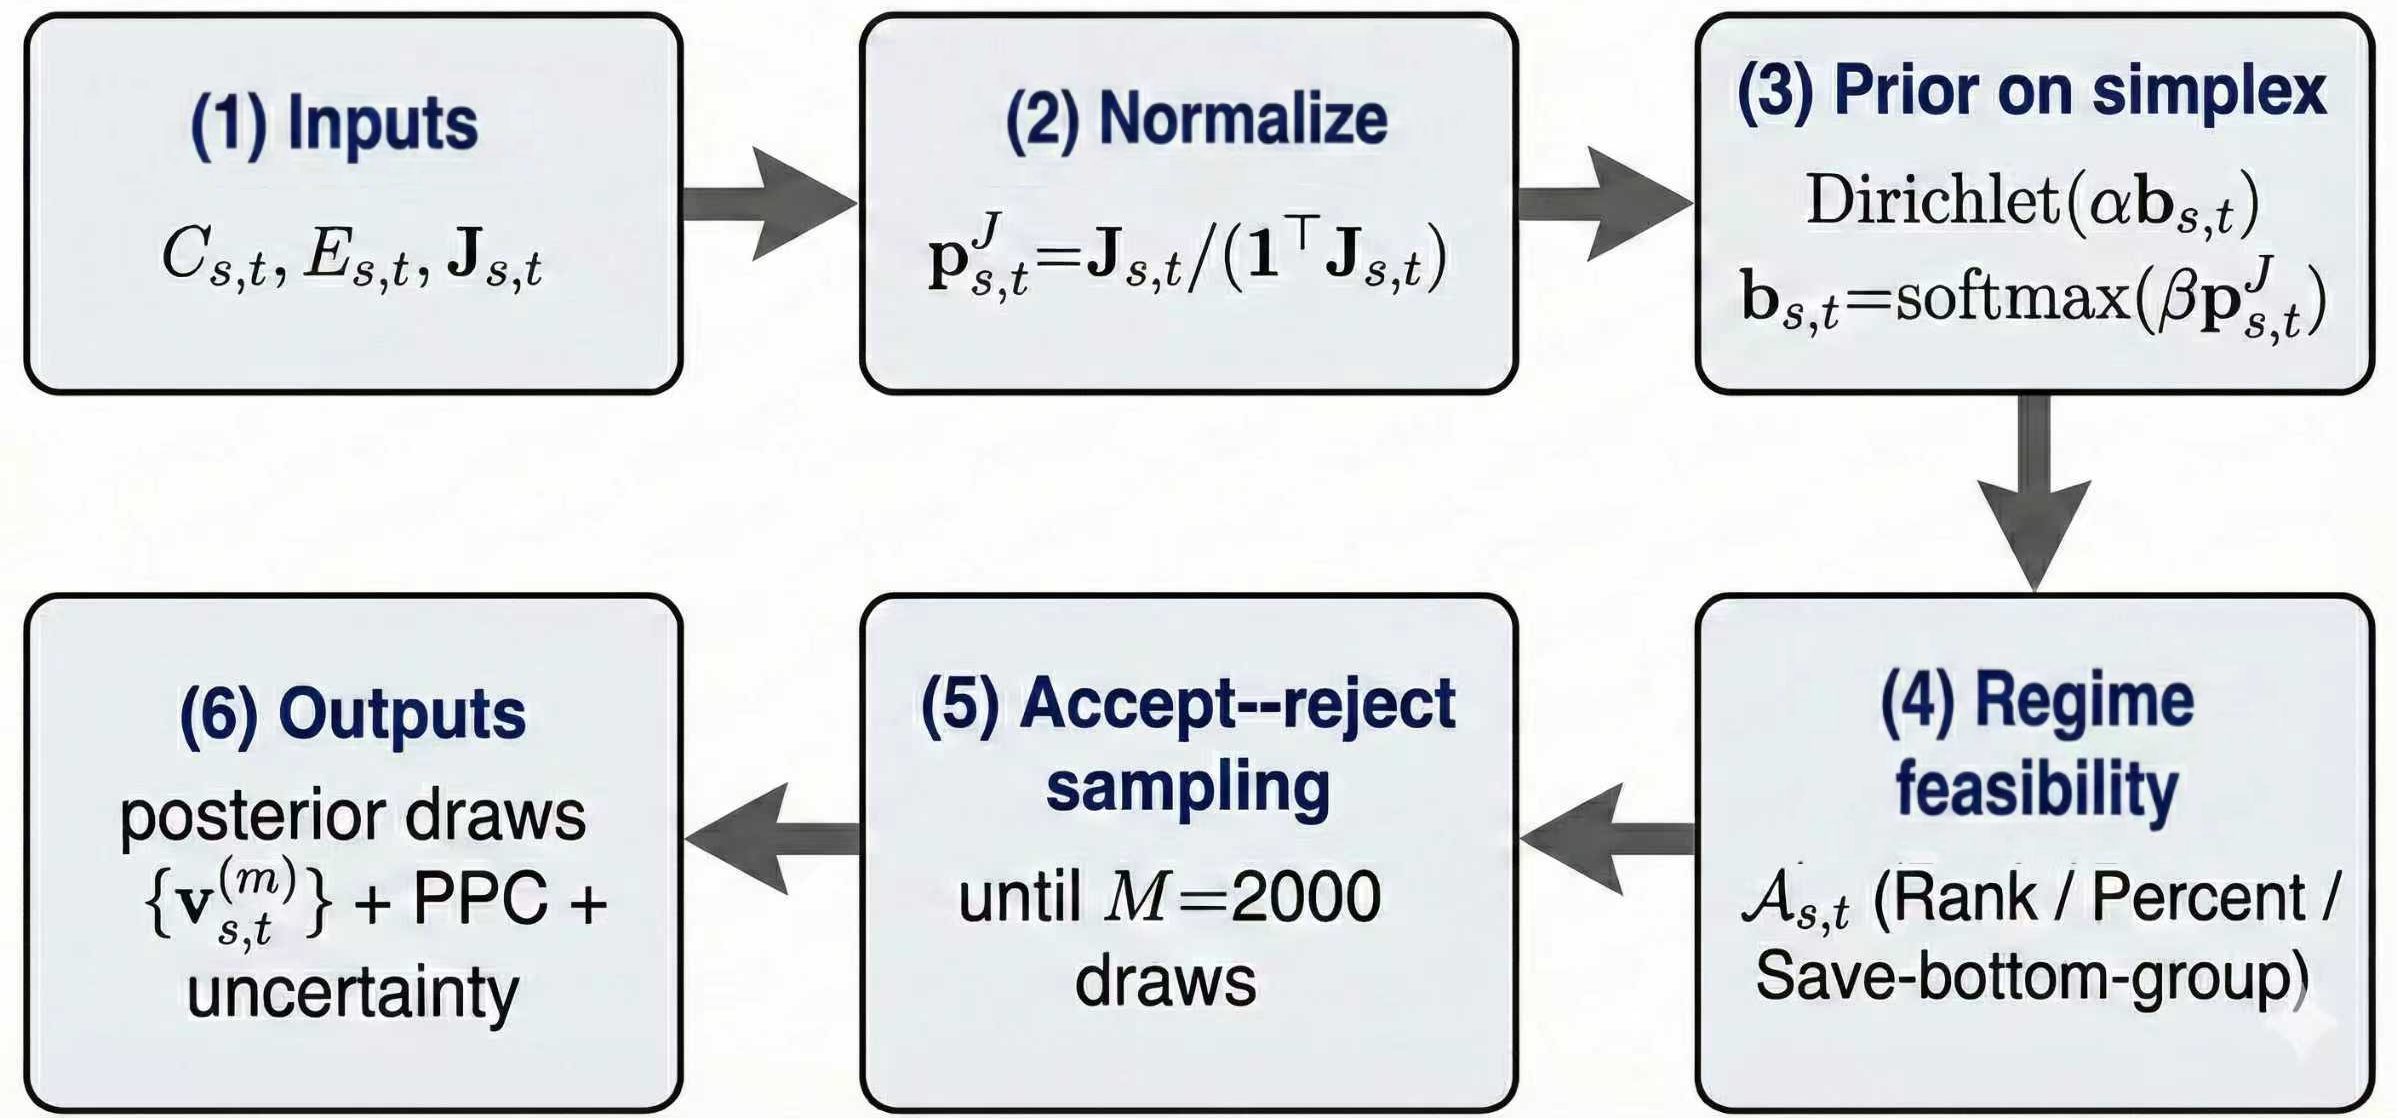
\includegraphics[width=0.52\textwidth]{figures/f1.png}
\caption{\textbf{Q1 pipeline (regime-aware inverse reconstruction).} Weekly inputs $(C_{s,t},E_{s,t},\mathbf{J}_{s,t})$ are mapped to posterior draws $\{\mathbf v^{(m)}_{s,t}\}_{m=1}^{M}$ via normalization (Eq.~\eqref{eq:q1_jshare}), a weak Dirichlet prior (Eq.~\eqref{eq:q1_prior}), and regime-specific feasibility (Eq.~\eqref{eq:q1_regimes}); diagnostics report PPC and uncertainty.}
\label{fig:q1_flow}
\end{figure}

% Gemini prompt:
% "Create a clean academic flowchart titled 'Q1 Regime-Aware Bayesian Inverse Vote Reconstruction'.
% Boxes (left-to-right): (1) Inputs: $C_{s,t}, E_{s,t}, \mathbf{J}_{s,t}$; (2) Normalize: $\mathbf p^J_{s,t}=\mathbf{J}_{s,t}/(\mathbf{1}^\top\mathbf{J}_{s,t})$;
% (3) Prior on simplex: Dirichlet$(\alpha \mathbf b_{s,t})$, $\mathbf b_{s,t}=\mathrm{softmax}(\beta\mathbf p^J_{s,t})$;
% (4) Regime feasibility $\mathcal A_{s,t}$ (Rank / Percent / Save-bottom-group);
% (5) Accept--reject sampling until $M=2000$ draws; (6) Outputs: posterior draws $\{\mathbf v^{(m)}_{s,t}\}$ + PPC + uncertainty.
% Use LaTeX-like math text, minimal color, professional style."

For each week $(s,t)$, we retain $M=2000$ accepted draws $\{\mathbf v^{(m)}_{s,t}\}_{m=1}^M$, utilizing the acceptance rate as a diagnostic metric to flag—rather than artificially correct—weeks exhibiting poor identifiability.

% ------------------------------------------------------------
% 3. Validation + uncertainty
% ------------------------------------------------------------
\subsection{Posterior Predictive Consistency and Diagnostics }
\label{sec:q1_val}

Finally, note that for weeks where accept--reject sampling succeeds, rule-consistency is satisfied \emph{by construction} for all retained draws. Therefore, rather than reporting the trivial within-draw consistency, we use a \textbf{week-level feasibility diagnostic} to quantify how often the historical outcome imposes a nonempty, practically sampleable feasible set.

Let $\mathcal{F}_{s,t}$ be the indicator that the sampling routine can obtain $M$ accepted draws under the regime constraint in Eq.~\eqref{eq:q1_regimes} within a fixed proposal budget. We define
\[
\mathcal{F}_{s,t}=\mathbf 1\!\left\{\text{obtain }M\text{ accepted draws for week }(s,t)\right\},
\qquad
\mathrm{PPC}=\frac{1}{|\mathcal{W}_{\mathrm{elim}}|}\sum_{(s,t)\in \mathcal{W}_{\mathrm{elim}}}\mathcal{F}_{s,t},
\]
where $\mathcal{W}_{\mathrm{elim}}$ denotes the set of elimination weeks. In our data, $\mathrm{PPC}=\mathbf{90.5\%}$, indicating that most elimination weeks admit a practically identifiable vote-share posterior under the observable constraints, while the remaining weeks are flagged as weakly identifiable and are excluded from mechanism-level comparisons.

For visualization only (not as ground truth), we summarize posterior uncertainty by the \textbf{posterior mean}
$\bar{\mathbf v}_{s,t}=\frac{1}{M}\sum_{m=1}^{M}\mathbf v^{(m)}_{s,t}$
and its \textbf{normalized entropy}
\[
H_{\mathrm{norm}}(\bar{\mathbf v}_{s,t})=\frac{-\sum_{i\in C_{s,t}}\bar v_{i,s,t}\log(\max\{\bar v_{i,s,t},\epsilon\})}{\log |C_{s,t}|}\in[0,1],
\]
with machine-level $\epsilon>0$ (e.g., $\epsilon=10^{-12}$) used only to avoid $\log 0$; it does not alter the simplex constraint in inference.

% ------------------------------------------------------------
% [FIGURE PLACEHOLDER Q1-F2] Diagnostics dashboard (PPC + uncertainty + two case weeks)
% Insertion location: after the PPC + uncertainty definitions above, before the diagnostic case text.
% Replaces: lengthy narrative descriptions of PPC variation and uncertainty structure across regimes.
% Data source (symbolic): posterior draws $\{\mathbf v^{(m)}_{s,t}\}$, judge shares $\mathbf p^J_{s,t}$, regime labels $R(s)$, PPC indicators $\mathbb I^{(m)}_{s,t}$.
% Figure attributes: multi-panel (a) PPC by season with regime boundaries; (b) box/violin of H_norm by regime; (c) two-week interval plot with $v$ CI + $p^J$ overlay.
% ------------------------------------------------------------
\begin{figure}[H]
\centering
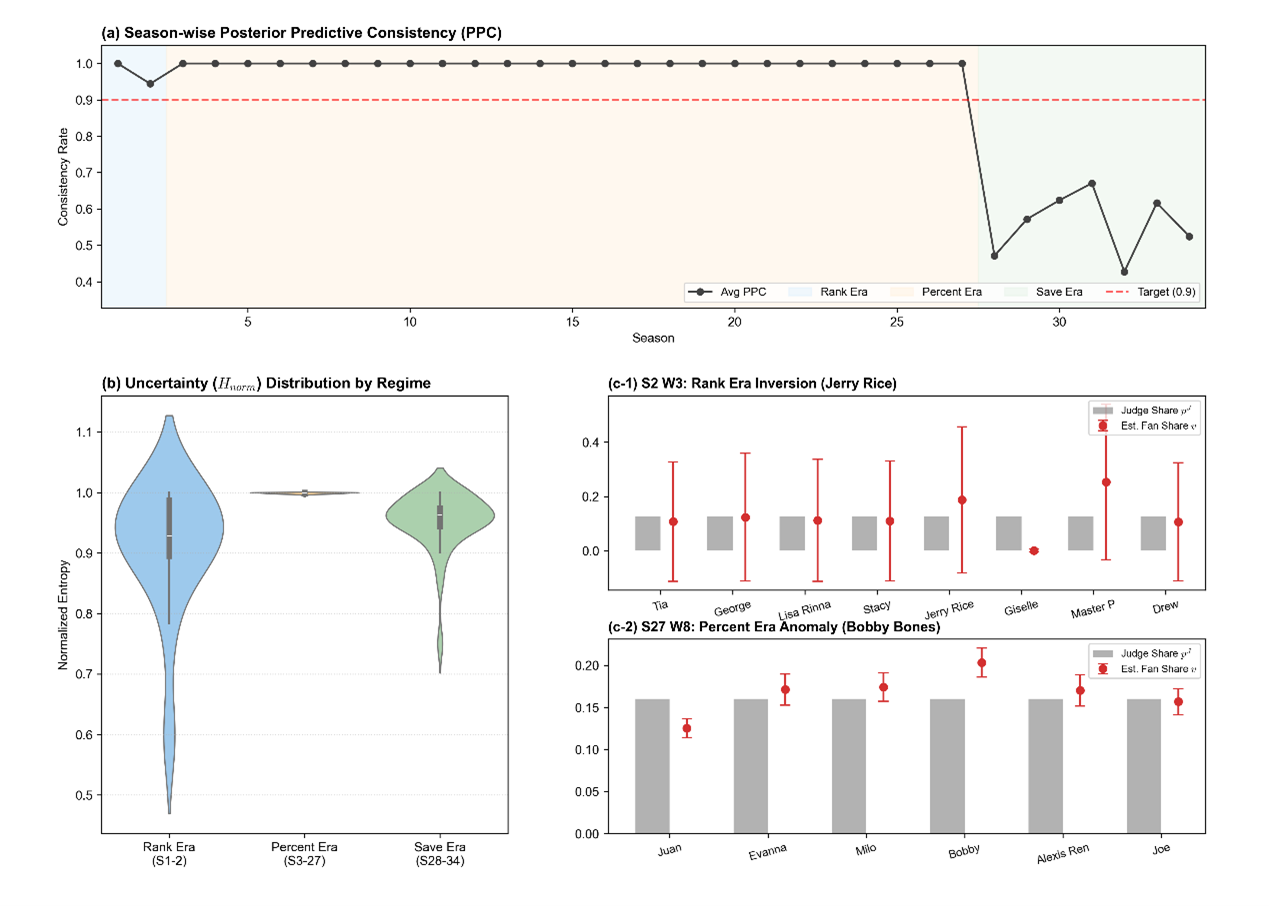
\includegraphics[width=0.62\textwidth]{figures/Q1figure2.png}
\caption{\textbf{Q1 posterior diagnostics.} (a) Season-wise PPC with regime boundaries; (b) $H_{\mathrm{norm}}(\bar{\mathbf v}_{s,t})$ by regime; (c) posterior intervals for S2W3 and S27W8 with $p^J_{i,s,t}$ overlays.}

\label{fig:q1_diag}
\end{figure}

% Gemini prompt:
% "Create a publication-style multi-panel figure titled 'Q1 Posterior Diagnostics'.
% Panel (a): line chart PPC by season (1–34), y-axis 'Mean PPC', with dashed vertical regime boundaries (1–2, 3–27a, 28a–34), annotate overall PPC=90.5%.
% Panel (b): boxplots of normalized entropy H_norm grouped by regime (Rank, Percent, Save). y-axis [0,1].
% Panel (c): two horizontal interval plots labeled 'S2 Week 3' and 'S27 Week 8'. For each, show several contestants with 95% credible intervals for vote share v; overlay judge share p^J as dots.
% Use academic font, minimal color, clean layout; no need to use real names in the mockup."

Our posterior analysis identifies distinct \textbf{Regime-Dependent Dynamics}. Season 2 (Jerry Rice) typifies judge--fan inversion where rank aggregation masks the magnitude of support, producing wider posteriors. Conversely, Season 27 (Bobby Bones) illustrates a \textbf{Systemic Anomaly} where extreme popularity concentrates posterior mass despite weak technical performance. These archetypes serve as critical stress tests for correcting anomalies without suppressing legitimate fan variance.

To facilitate downstream comparison, we export this reconstruction as a rigorous \textbf{Probabilistic Baseline}. For each week $(s,t)$, we store the full matrix of posterior draws $\mathbf V_{s,t}\in\mathbb{R}^{M\times |C_{s,t}|}$ together with derived diagnostics (credible intervals, PPC). This ensures that Q2 compares aggregation rules under identical uncertainty conditions, treating these draws as the sole admissible interface for fan support.

Finally, the analysis reveals a \textbf{Structural Separation} inherent in the Save Era, distinguishing the \emph{baseline aggregator} from the \emph{safety layer}. This insight grounds the **Modular Safety Network (MSN)** proposed in Q4: a structured composition that combines a stable percent baseline with minimal bottom-two protection, introducing fan-facing features only after establishing baseline stability.


% ============================================================
% Q2: Systemic Sensitivity & Rule Comparison (Rewritten)
% Aligned with Q4 Style (PAGS/Circuit-Breaker Terminology)
% ============================================================
\section{\textbf{Comparative Evaluation of Voting Aggregation Rules and the Judges' Save}  }
\label{sec:q2}

\subsection{The Within-Week Counterfactual Simulation Design }
\label{sec:q2_design}

To isolate the structural properties of aggregation rules from the path dependence of the competition (where one elimination alters all future contestant pools), we adopt a \emph{within-week counterfactual framework}.
For every historical week $(s,t)$, the realized set of active contestants $C_{s,t}$ and the judges' dynamic scoring vector $\mathbf{J}_{s,t}$ are held fixed. The latent fan support is treated not as a point estimate, but as a distribution using the posterior samples $\{\mathbf{v}^{(m)}_{s,t}\}_{m=1}^{M}$ inferred in Model I (Q1), with $M=2000$.
This approach allows for the propagation of uncertainty through the aggregation mechanism, yielding probabilistic estimates of elimination risks under alternative rules rather than deterministic binary outcomes.

\subsection{Mathematical Formalization of Aggregation Regimes}
\label{sec:q2_formalization}

Let $m_{s,t}$ denote the number of contestants to be eliminated in week $(s,t)$. We formalize the two primary historical aggregation rules and the ``Save'' mechanism as distinct mapping functions $E: \mathbb{R}^{|C_{s,t}|} \to 2^{C_{s,t}}$.

\noindent\textbf{Regime A: Percentage Aggregation (Percent)}
\\
The Percentage rule aggregates normalized shares. Let $p^{J}_{i,s,t}$ be the judge-share derived from $\mathbf{J}_{s,t}$, and let $\mathbf v_{s,t}\in\Delta^{|C_{s,t}|-1}$ denote latent \emph{fan vote shares} (not absolute vote counts). The composite score for contestant $i$ is $c_{i,s,t}=p^{J}_{i,s,t}+v_{i,s,t}$.
The elimination set is defined as the subset of size $m_{s,t}$ with the lowest composite scores:
\begin{equation}
    E_{s,t}^{\mathrm{Pct}}(\mathbf{v}_{s,t}) = \mathrm{Bottom}_{m_{s,t}}\left( \mathbf{p}^{J}_{s,t} + \mathbf{v}_{s,t} \right).
\end{equation}

\noindent\textbf{Regime B: Ordinal Rank Aggregation (Rank)}
\\
The Rank rule aggregates ordinal positions. Let $\operatorname{rank}_{\downarrow}(\cdot)$ be the descending rank operator, where rank $1$ denotes the highest score (best performance) and larger ranks indicate worse performance.

Define $r_{i,s,t}^J=\operatorname{rank}_{\downarrow}(J_{i,s,t})$ and $r_{i,s,t}^F=\operatorname{rank}_{\downarrow}(v_{i,s,t})$ as the judge and fan ranks of contestant $i$. The rank-sum disadvantage is $B_{i,s,t}=r_{i,s,t}^J+r_{i,s,t}^F$. Define $\mathrm{Worst}_{m}(\cdot)$ as selecting the indices of the $m$ largest entries (ties broken deterministically). The elimination set corresponds to the $m_{s,t}$ largest rank sums:
\begin{equation}
    E_{s,t}^{\mathrm{Rank}}(\mathbf{v}_{s,t}) = \mathrm{Worst}_{m_{s,t}}\left( \mathbf{r}_{s,t}^J + \mathbf{r}_{s,t}^F(\mathbf{v}_{s,t}) \right).
\end{equation}



\noindent\textbf{Regime C: The Idealized Meritocratic Save (IMS)}
\\
We introduce an \emph{Idealized Meritocratic Save (IMS)} as a \textbf{ceiling benchmark} on how much a save layer \emph{could} correct fan-driven eliminations under purely technical decision-making. Since DWTS is an entertainment program, real judges may deviate from merit; thus IMS is \emph{not} a behavioral model, but an upper bound that brackets the maximum potential technical correction. 

Such deviations can be interpreted as an additive disturbance in the save choice (set to zero here to preserve interpretability and parsimony).


Given a base rule $R\in\{\mathrm{Pct},\mathrm{Rank}\}$, let $\mathbf z^R_{s,t}(\mathbf v)$ denote its baseline decision score vector on week $(s,t)$:
\[
\mathbf z^{\mathrm{Pct}}_{s,t}(\mathbf v)=\mathbf p^J_{s,t}+\mathbf v,\qquad
\mathbf z^{\mathrm{Rank}}_{s,t}(\mathbf v)=\mathbf r^J_{s,t}+\mathbf r^F_{s,t}(\mathbf v),
\]
where larger $\mathbf z^{\mathrm{Rank}}$ indicates worse standing (rank-sum disadvantage).
Define the Bottom-2 set under rule $R$ as $\mathrm{Bottom2}(\mathbf z^R_{s,t}(\mathbf v))$ using the appropriate ordering. IMS then eliminates the weaker technical performer within this bottom tier:
\begin{equation}
E_{s,t}^{R+\mathrm{IMS}}(\mathbf{v}_{s,t}) =
\left\{ \arg\min_{k \in \mathrm{Bottom2}(\mathbf{z}^R_{s,t}(\mathbf{v}_{s,t}))} J_{k,s,t} \right\}.
\end{equation}


\subsection{Uncertainty Propagation and Comparative Metric Formulation }
\label{sec:q2_metrics}

Consistent with the uncertainty propagation in Q1, all comparative metrics are computed as expectations over the posterior draws.

\paragraph{Disagreement Probability ($P_{\mathrm{diff}}$).}
The probability that the two regimes yield different elimination sets:
\begin{equation}
    P_{\mathrm{diff}}(s,t) = \frac{1}{M} \sum_{m=1}^M \mathbf{1}\left\{ E_{s,t}^{\mathrm{Pct}}(\mathbf{v}^{(m)}_{s,t}) \neq E_{s,t}^{\mathrm{Rank}}(\mathbf{v}^{(m)}_{s,t}) \right\}.
\end{equation}

\paragraph{Expected Symmetric Difference ($D_{\mathrm{exp}}$).}
To measure the magnitude of divergence, we compute the expected cardinality of the symmetric difference:
\begin{equation}
    D_{\mathrm{exp}}(s,t) = \mathbb{E}\left[ \left| E_{s,t}^{\mathrm{Pct}} \Delta E_{s,t}^{\mathrm{Rank}} \right| \right].
\end{equation}

\paragraph{Fan Alignment Index (FAI).}
To quantify the bias of a rule $R$ toward audience agency versus technical merit, we define the FAI. Let $i_F^*$ be the fan-bottom contestant and $i_J^*$ be the judge-bottom contestant.
\begin{equation}
    \mathrm{FAI}^R(s,t) = \Pr(i_F^* \in E^R_{s,t}) - \Pr(i_J^* \in E^R_{s,t}).
\end{equation}
$\mathrm{FAI} > 0$ indicates the mechanism is more likely to eliminate the fan-bottom contestant ($i_F^*$), reflecting stronger fan agency in the marginal elimination decision. In contrast, $\mathrm{FAI} < 0$ indicates a technical-correction tendency: the mechanism is more likely to eliminate the judge-bottom contestant ($i_J^*$) even when the fan-bottom differs, thereby reducing purely popularity-driven eliminations.


\paragraph{Global Consistency ($\rho$).}
Beyond binary elimination, we measure the structural alignment of the entire leaderboard using the Spearman rank correlation $\rho_S$ between the rule-implied order and the latent fan preference order.

\subsection{Structural Volatility and Historical Evolution Analysis }
\label{sec:q2_results}

\subsubsection{Aggregated Sensitivity Analysis}
The counterfactual simulation reveals that the choice of aggregation mechanism is non-trivial. Across 264 elimination weeks, the Rank and Percentage rules produce divergent elimination outcomes in \textbf{26.0\%} of cases ($P_{\mathrm{diff}} = 0.260$), with an average symmetric difference of $D_{\mathrm{exp}} = 0.485$.
This confirms that for a quarter of the show's history, the elimination outcome was determined not by performance or popularity but by the mathematical properties of the aggregation formula.

\begin{figure}[H]
    \centering
    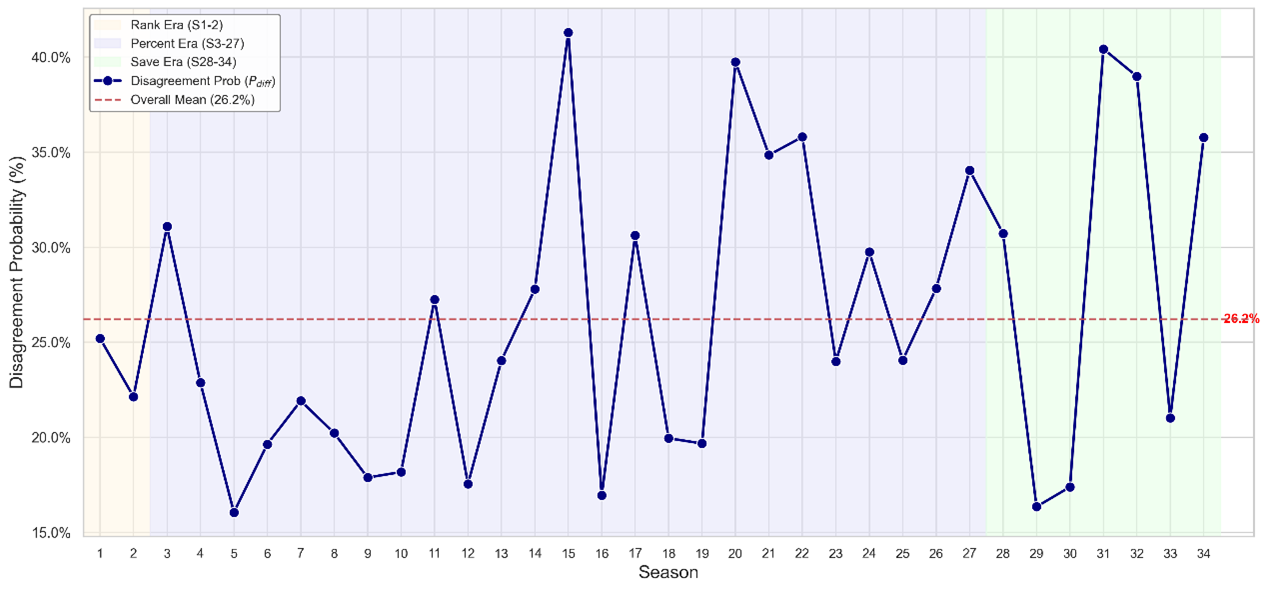
\includegraphics[width=0.55\textwidth]{Q2.4.png}
    \caption{\textbf{Global consistency with fan intent.} Distribution of $\rho$ under Percent (left) and Rank (right); Percent exhibits higher average consistency ($\bar{\rho}=0.765$ vs.\ $0.678$).}
    \label{fig:rho_dist}
\end{figure}

\subsubsection{Era-Dependent Structural Shifts}
Table \ref{tab:phase_metrics} disaggregates these metrics by historical era. Two distinct regimes emerge:

\begin{enumerate}
    \item \textbf{The Agency Regime (S3--27):} Under the Percentage rule, the system exhibits high fan alignment ($\mathrm{FAI}_{\mathrm{Pct}} = 0.277$) and global consistency ($\rho_{\mathrm{Pct}} = 0.765$). This mechanism efficiently translates vote share into survival probability.
    \item \textbf{The Technical Correction Regime (S28--34):} The introduction of the Save mechanism (modeled via IMS) inverts the alignment index ($\mathrm{FAI} < 0$). This is not a numerical anomaly but a quantified structural shift: the two-stage decision process increases the probability that the \emph{technical} bottom ($i_J^*$) is eliminated compared to the \emph{fan} bottom ($i_F^*$).
\end{enumerate}

\begin{table}[H]
    \centering
    \caption{\textbf{Structural Metrics by Historical Era.} Note the inversion of FAI in the Save Era (S28--34), indicating a shift toward meritocratic protection.}
    \label{tab:phase_metrics}
    \small
    \setlength{\tabcolsep}{4pt}
    \begin{tabular}{lccccccc}
        \toprule
        \textbf{Era} & \textbf{Weeks} & \textbf{$P_{\mathrm{diff}}$} & \textbf{$D_{\mathrm{exp}}$} & \textbf{$\mathrm{FAI}_{\mathrm{Pct}}$} & \textbf{$\mathrm{FAI}_{\mathrm{Rank}}$} & \textbf{$\rho_{\mathrm{Pct}}$} & \textbf{$\rho_{\mathrm{Rank}}$} \\
        \midrule
        Rank Era (S1--2)      & 10  & 0.231 & 0.461 & 0.156  & 0.425 & \textbf{0.861}& 0.682 \\
        Percent Era (S3--27)  & 198 & 0.253 & 0.467 & 0.277  & 0.142 & \textbf{0.749}& 0.669 \\
        Save Era (S28--34)    & 56  & \textbf{0.291}& \textbf{0.549}& -0.047 & 0.327 & \textbf{0.804}& 0.710 \\
        \bottomrule
    \end{tabular}
\end{table}

\subsection{Quantification of the IMS Circuit Breaker Effect }
\label{sec:q2_ims}

The IMS baseline isolates the marginal effect of the ``Judges' Save.'' In the 47 weeks where the mechanism reduces to ``Bottom-2 + Re-decision,'' the inclusion of IMS induces a significant negative shift in fan alignment:
\begin{equation}
    \Delta \mathrm{FAI}_{\mathrm{Rank}} = -0.425 \quad \text{and} \quad \Delta \mathrm{FAI}_{\mathrm{Pct}} = -0.055.
\end{equation}
This quantifies the Save mechanism as a \emph{technical circuit breaker}: it systematically overrides fan intent when that intent conflicts with the judges' technical assessment in the bottom tier. The effect is particularly pronounced when superimposed on the Rank mechanism.

\begin{figure}[H]
    \centering
    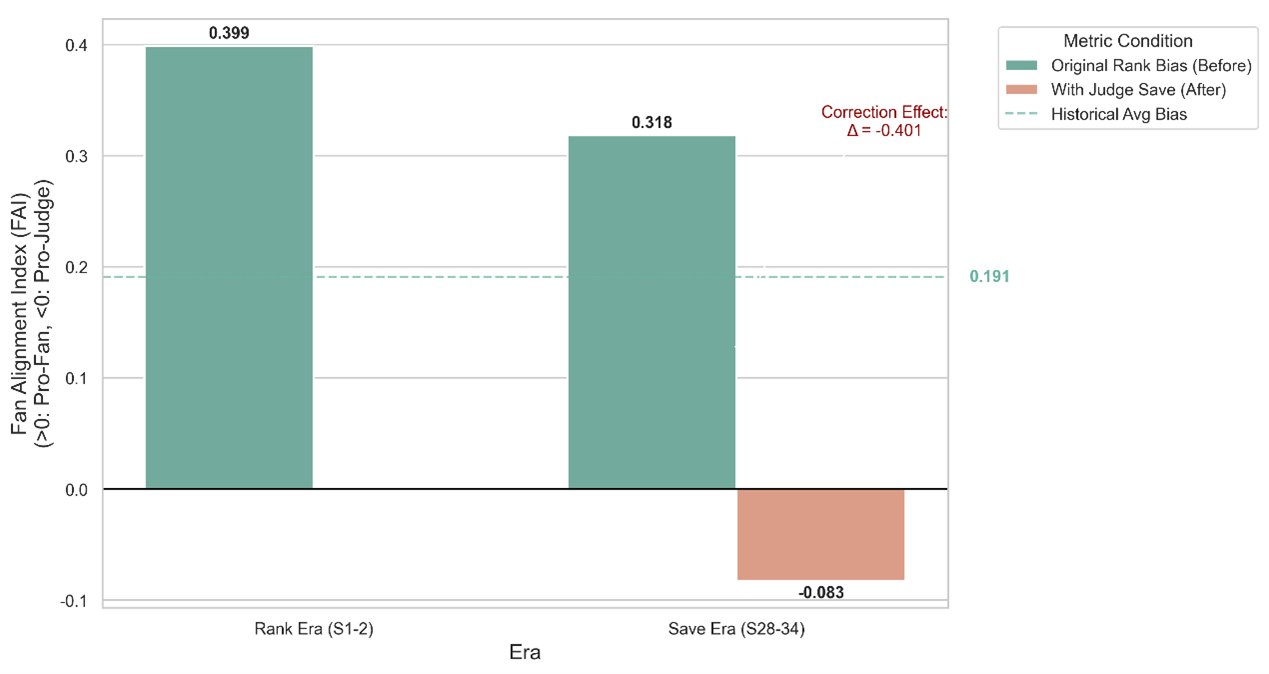
\includegraphics[width=0.72\textwidth]{Q2.3.png}
    \caption{\textbf{Evolution of Fairness (FAI) and Consistency ($\rho$) Across Eras.} The dashed lines represent global historical means. The suppression of FAI in the S28-34 era reflects the active intervention of the Save mechanism.}
    \label{fig:fai_evolution}
\end{figure}

\subsection{Counterfactual Stress Testing of Controversial Profiles }
\label{sec:q2_cases}

To validate the model at the micro-level, we examine specific ``controversial'' contestants—defined as those with high disagreement between judge scores and fan support ($G_i = \mathbb{E}[r^J - r^F]$). We compare their elimination probabilities $p_{\mathrm{elim}}$ in critical weeks under different regimes.

As shown in Table \ref{tab:controversy}, the choice of mechanism is determinant for certain profiles:

\begin{table}[H]
    \centering
    \caption{\textbf{Counterfactual Risk Assessment for High-Variance Profiles.} $\Delta p$ denotes the maximum difference in elimination probability between Rank and Percentage rules in the critical week $t^*$.}
    \label{tab:controversy}
    \footnotesize
    \setlength{\tabcolsep}{3.5pt}
    \renewcommand{\arraystretch}{1.02}
    \begin{tabular}{lcccccc}
        \toprule
        \textbf{Contestant (Season)} & \textbf{Week $t^*$} & \textbf{$p_{\mathrm{elim}}^{\mathrm{Pct}}$} & \textbf{$p_{\mathrm{elim}}^{\mathrm{Rank}}$} & \textbf{$\Delta p$} & \textbf{$p_{\mathrm{elim}}^{\mathrm{Rank+IMS}}$} & \textbf{Divergence $G_i$} \\
        \midrule
        Jerry Rice (S2)      & 3 & \textbf{0.296}& 0.002 & {0.294}& \textbf{0.353}& 1.701 \\
        Billy Ray Cyrus (S4) & 8 & \textbf{0.900}& 0.558 & \textbf{0.341} & 0.822 & 2.088 \\
        Bristol Palin (S11)  & 5 & \textbf{0.124}& 0.087 & 0.036          & \textbf{0.298}& 2.508 \\
        Bobby Bones (S27)    & 1 & \textbf{0.014}& 0.001 & 0.013          & 0.000 & \textbf{3.048}\\
        \bottomrule
    \end{tabular}
\end{table}

\begin{itemize}
    \item \textbf{Type I Divergence (e.g., Jerry Rice, S2):} A massive risk differential ($\Delta p = 0.294$) exists. The Rank mechanism almost guarantees safety ($p=0.002$) due to rank-buffering, whereas Percentage exposes the contestant to significant risk ($p=0.296$).
    \item \textbf{Type II Convergence (e.g., Bobby Bones, S27):} Despite high controversy ($G_i=3.048$), the fan support is so overwhelming that $\Delta p \approx 0$. Here, neither base mechanism suffices to correct the meritocratic deviation, necessitating the stronger ``circuit breaker'' interventions proposed in Section 6 (PAGS).
\end{itemize}




\begin{figure}[H]  % [H] 让图片固定在这里，不再跑到页面顶部
    \centering
    % \makebox 强制让图片在整个文本宽度内居中，消除任何缩进干扰
    \makebox[\textwidth][c]{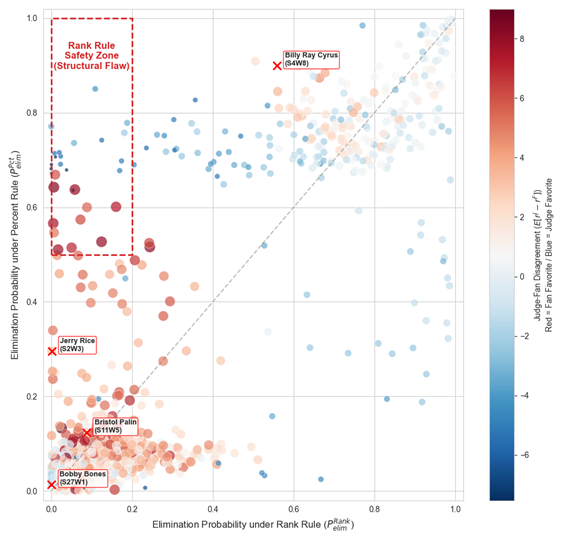
\includegraphics[width=0.48\textwidth]{figures/risk_conflict_map.png}}
   \caption{\textbf{Risk conflict map (Rank vs.\ Percent).} Each point is a contestant-week; x-axis: $p_{\mathrm{elim}}^{\mathrm{Rank}}$, y-axis: $p_{\mathrm{elim}}^{\mathrm{Pct}}$. The highlighted top-left region marks cases that are high-risk under Percent but protected under Rank.}

    \label{fig:risk_conflict_map}
\end{figure}


\subsection{Synthesis of the Merit-Agency Trade-off }
The comparative analysis suggests a fundamental trade-off that informs the design in Section \ref{sec:q4}:
\begin{enumerate}
    \item If the objective is \textbf{Fan Agency (Engagement)}, the Percentage rule is superior ($\rho_{\mathrm{Pct}} > \rho_{\mathrm{Rank}}$), as it preserves the magnitude of popular support.
    \item If the objective is \textbf{Technical Stability}, the Rank mechanism dampens volatility but creates arbitrary safety zones for controversial figures (e.g., Jerry Rice).
    \item To achieve \textbf{Meritocratic Integrity} without sacrificing engagement, a simple rule change is insufficient. The ``Save'' (IMS) provides necessary correction ($\Delta \mathrm{FAI} < 0$), but its opaque application creates consistency issues. This conclusion directly motivates the transparent, parametric guardrails of the PAGS architecture proposed in Q4.
\end{enumerate}


% ============================================================
% Q3: Multidimensional Attribution Analysis (compressed, O-level)
% Keep existing figures Q3.1--Q3.4
% ============================================================

\section{Quantifying Judges' and Audience Impacts on Elimination Risk}

\label{sec:q3}

\subsection{Latent Uncertainty Propagation to Downstream Models }
\label{sec:q3_inputs}

To propagate the uncertainty inherent in the inverse reconstruction, we bypass deterministic point estimates and instead utilize the full posterior ensemble $\{\mathbf v^{(m)}_{s,t}\}_{m=1}^{M}$ ($M=2000$), where each $\mathbf v^{(m)}_{s,t}$ satisfies the simplex constraint $\sum_{i\in C_{s,t}} v^{(m)}_{i,s,t}=1$. By treating each draw as a completed popularity scenario and pooling downstream estimates via Rubin's multiple-imputation rules , we ensure that subsequent analyses reflect the true ambiguity of the latent votes rather than the bias of plug-in means.
\paragraph{Pooling rule (Rubin's MI).}
Let $\theta^{(m)}$ denote an estimate computed under draw $m$ with estimated variance $U^{(m)}$ (e.g., from the fitted model). Rubin's rules pool uncertainty as
\[
\bar\theta=\frac{1}{M}\sum_{m=1}^M \theta^{(m)},\quad
\bar U=\frac{1}{M}\sum_{m=1}^M U^{(m)},\quad
B=\frac{1}{M-1}\sum_{m=1}^M\left(\theta^{(m)}-\bar\theta\right)^2,\quad
T=\bar U+\left(1+\frac{1}{M}\right)B,
\]
and we report $\bar\theta\pm 1.96\sqrt{T}$ when approximate normality is adequate.


\begin{definition}[Attribution Challenge]
Elimination outcomes are driven by heterogeneous channels: a meritocratic channel (judges) and a democratic channel (fans).
The attribution challenge is to quantify the conditional contribution of professional partners after controlling for celebrity traits and season-week context,
without extrapolating counterfactual post-elimination trajectories.
\end{definition}

\begin{definition}[Meritocratic Signal]
For $i\in C_{s,t}$, the observed judge input is $J_{i,s,t}$ (field \texttt{wt\_avg}).
Define within-week standardized judge performance
\[
Y^J_{i,s,t}=\frac{J_{i,s,t}-\bar J_{s,t}}{\sigma_{J,s,t}},\qquad
\bar J_{s,t}=\frac{1}{|C_{s,t}|}\sum_{k\in C_{s,t}}J_{k,s,t},
\]
where $\sigma_{J,s,t}$ is the sample standard deviation of $\{J_{k,s,t}:k\in C_{s,t}\}$.
\end{definition}

\begin{definition}[Democratic Signal in Euclidean Geometry]
For each draw $m$, fan support lies on the simplex and is mapped to Euclidean space by the centered log-ratio (CLR). To ensure the log transform is well-defined, we apply a machine-level pseudocount and renormalize:
\[
v^{\dagger(m)}_{i,s,t}=\max\{v^{(m)}_{i,s,t},\epsilon\},\qquad
\tilde v^{(m)}_{i,s,t}=\frac{v^{\dagger(m)}_{i,s,t}}{\sum_{k\in C_{s,t}} v^{\dagger(m)}_{k,s,t}}.
\]
We then compute
\[
\mathrm{clr}\!\left(\tilde v^{(m)}_{i,s,t}\right)=
\log \tilde v^{(m)}_{i,s,t}-\frac{1}{|C_{s,t}|}\sum_{k\in C_{s,t}}\log \tilde v^{(m)}_{k,s,t}.
\]

Define within-week standardized popularity response
\[
Y^{V(m)}_{i,s,t}=
\frac{\mathrm{clr}(v^{(m)}_{i,s,t})-\overline{\mathrm{clr}}^{(m)}_{s,t}}{\sigma^{(m)}_{\mathrm{clr},s,t}},
\]
so that $Y^{V(m)}_{i,s,t}$ and $Y^{J}_{i,s,t}$ are comparable on a one-standard-deviation scale.
\end{definition}

To isolate the impact of professional partners while strictly preventing data leakage, we construct a \textbf{Leakage-Controlled Pro Profile} $\mathbf z_{d,s}=(\mathrm{Tenure}_d,\ \mu^{J,\mathrm{LOSO}}_{d,-s})^\top$, where $\mu^{J,\mathrm{LOSO}}_{d,-s}$ represents the partner's historical performance averaged over all seasons $s'\neq s$ (a \textbf{Leave-One-Season-Out} estimator). Simultaneously, we account for contestant heterogeneity via \textbf{Celebrity Covariates} $\mathbf x_i$, comprising centered age and stabilized industry dummies (with rare categories merged into \texttt{Other}).

\subsection{The Judge-Fan-Survival Three-Channel Architecture }
\label{sec:q3_models}

To disentangle the mechanisms conflated in the raw elimination outcomes, we structurally model three distinct components: the judges' technical assessment, the fan preference conditional on observed performance, and the stochastic advancement dynamics governing the risk set.

\paragraph{Channel J: technical assessment (judges).}
Let $Y^J_{i,s,t}$ be the within-week standardized judge score. We use a mixed-effects structure that isolates (a) celebrity traits, (b) interpretable pro profile effects, and (c) residual partner heterogeneity:
\begin{equation}
Y^J_{i,s,t}
=
\mathbf x_i^\top \boldsymbol\beta^J
+
\mathbf z_{d(i),s}^\top \boldsymbol\eta^J
+
\phi_{\mathrm{era}(s),t}
+
u_s^J
+
b^J_{d(i)}
+
\epsilon^J_{i,s,t}.
\label{eq:q3_judge_lmm}
\end{equation}
\noindent\textbf{Notation (model components).}
$\mathbf x_i$ are celebrity covariates; $d(i)$ maps celebrity $i$ to professional partner $d$; $\mathbf z_{d(i),s}$ is the leakage-controlled pro profile; $\phi_{\mathrm{era}(s),t}$ is an era-by-week fixed effect; $u_s^{J/V}$ are season random intercepts; $b_{d}^{J/V}$ are pro-dancer random effects; $\epsilon$ are idiosyncratic errors; and $\kappa_J,\kappa_V$ quantify the protective effects of technical merit and popularity in the hazard.


\paragraph{Channel V: popularity conditional on performance (fans).}
For each draw $m$, let $Y^{V(m)}_{i,s,t}$ denote the standardized log-ratio popularity response. Conditioning on contemporaneous performance prevents ``good dancing'' from being misread as ``being liked'':
\begin{equation}
Y^{V(m)}_{i,s,t}
=
\mathbf x_i^\top \boldsymbol\beta^V
+
\mathbf z_{d(i),s}^\top \boldsymbol\eta^V
+
\gamma\, Y^J_{i,s,t}
+
u_s^V
+
b^V_{d(i)}
+
\epsilon^{V(m)}_{i,s,t}.
\label{eq:q3_fan_lmm}
\end{equation}

\paragraph{Channel H: advancement dynamics (discrete-time survival).}
Let $h^{(m)}_{i,s,t}$ be the elimination hazard at week $t$ given survival to $t{-}1$.
A discrete-time hazard specification links advancement to both technical and popularity signals\footnote{Discrete-time hazard modeling follows standard survival texts.}:
\begin{equation}
\mathrm{logit}\!\left(h^{(m)}_{i,s,t}\right)
=
\delta_t
+
\mathbf x_i^\top \boldsymbol\beta^H
+
\kappa_J\, Y^J_{i,s,t}
+
\kappa_V\, Y^{V(m)}_{i,s,t}.
\label{eq:q3_hazard}
\end{equation}
where $\delta_t$ is the week-specific baseline log-odds (time effect).

\subsection{Visual Analysis of Findings and Robustness Checks }
\label{sec:q3_findings}

Crucially, our analysis reveals that \textbf{Fan and Judge Criteria} decouple along interpretable dimensions (Figure~\ref{fig:q3_coef_contrast}). While technical scoring exhibits a sharp negative gradient with age, conditional fan preference is attenuated and frequently reverses direction. This divergence provides quantitative evidence of a \textbf{Sympathy-Compensation Pattern}, where audience support actively counterbalances technical deficits rather than purely tracking performance.

\begin{figure}[t]
  \centering
  \begin{subfigure}[t]{0.53\textwidth}
    \centering
    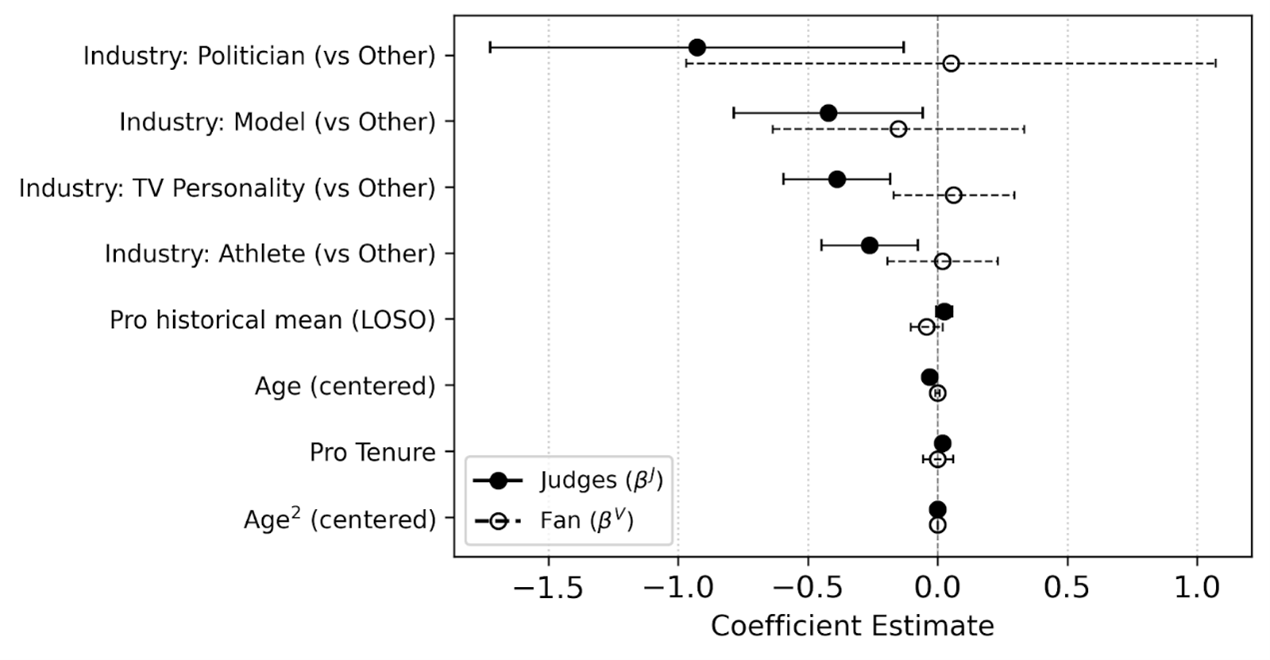
\includegraphics[width=\textwidth]{figures/Q3.1.png}
    \caption{Fixed-effect estimates (standardized) with 95\% intervals for the judge channel ($\boldsymbol\beta^J$) and the fan channel ($\boldsymbol\beta^V$), with fan-side uncertainty pooled over $M=2000$ Q1 posterior vote draws.}
    \label{fig:q3_coef_contrast}
  \end{subfigure}
  \hfill
  \begin{subfigure}[t]{0.43\textwidth}
    \centering
    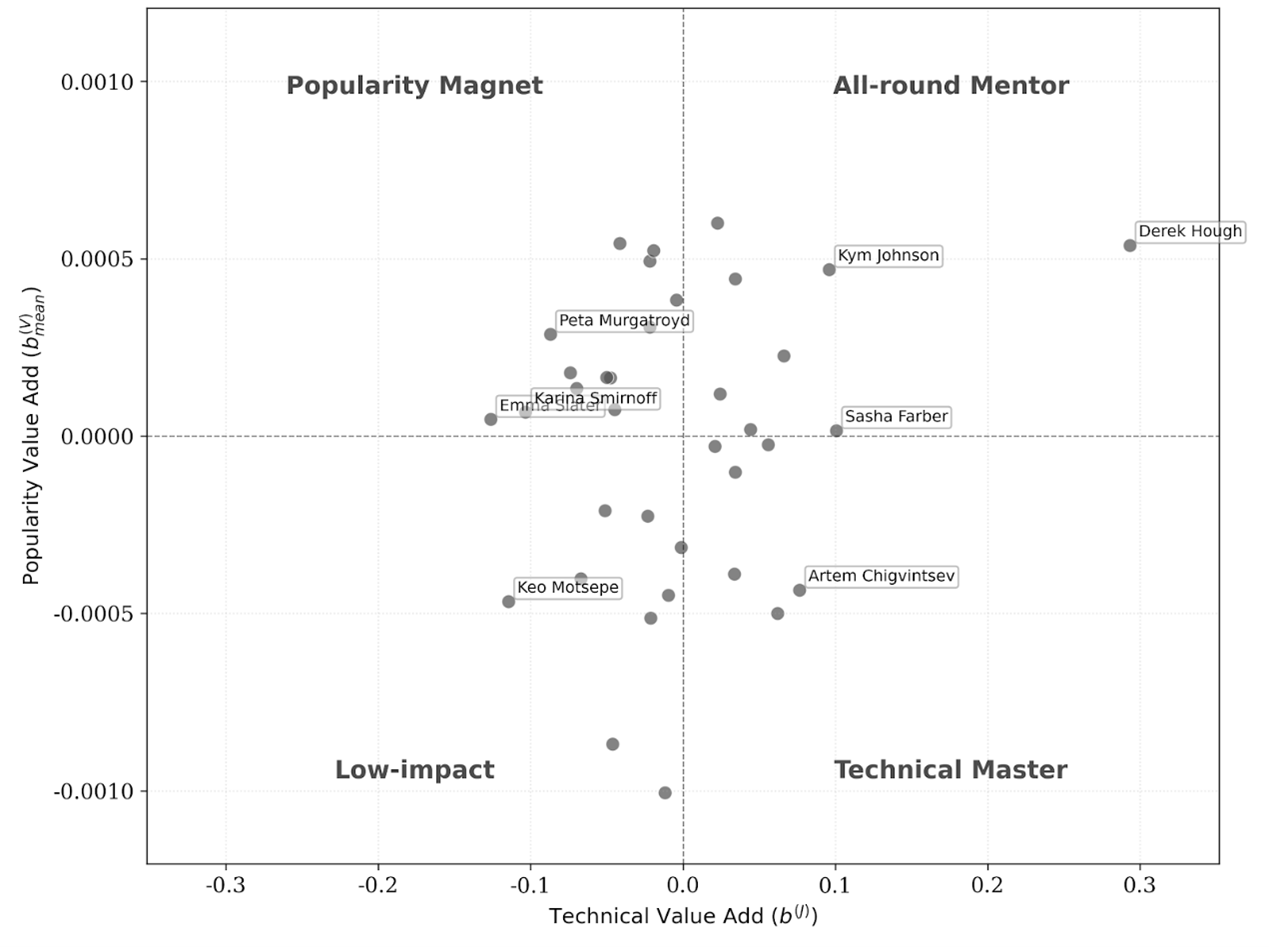
\includegraphics[width=\textwidth]{figures/Q3.2.png}
    \caption{Each professional is positioned by estimated residual technical value add ($b^{(J)}$) and residual popularity value add ($b^{(V)}$), separating ``technical uplift'' from ``popularity transfer'' beyond observed covariates.}
    \label{fig:q3_pro_scatter}
  \end{subfigure}
  \caption{\textbf{Cross-channel contrast and pro-dancer value add.}}
  \label{fig:q3_side_by_side}
\end{figure}


Furthermore, Figure~\ref{fig:q3_pro_scatter} demonstrates that professional partner effects are strongly \textbf{Channel-Dependent}, distinguishing technical specialists (positive $b^{(J)}$) from popularity multipliers (positive $b^{(V)}$) and revealing a heterogeneous ``value add'' that transcends simple tenure metrics.



Finally, the hazard estimates in Fig.~\ref{fig:q3_or_forest} corroborate that advancement is governed by a robust \textbf{Dual-Signal Mechanism}. Both technical merit ($Y^J$) and audience support ($Y^{V(m)}$) exert significant protective effects, confirming that elimination remains a joint decision process even after adjusting for demographic covariates and baseline weekly risk.

\begin{figure}[H]
  \centering
  \begin{subfigure}[t]{0.43\textwidth}
    \centering
    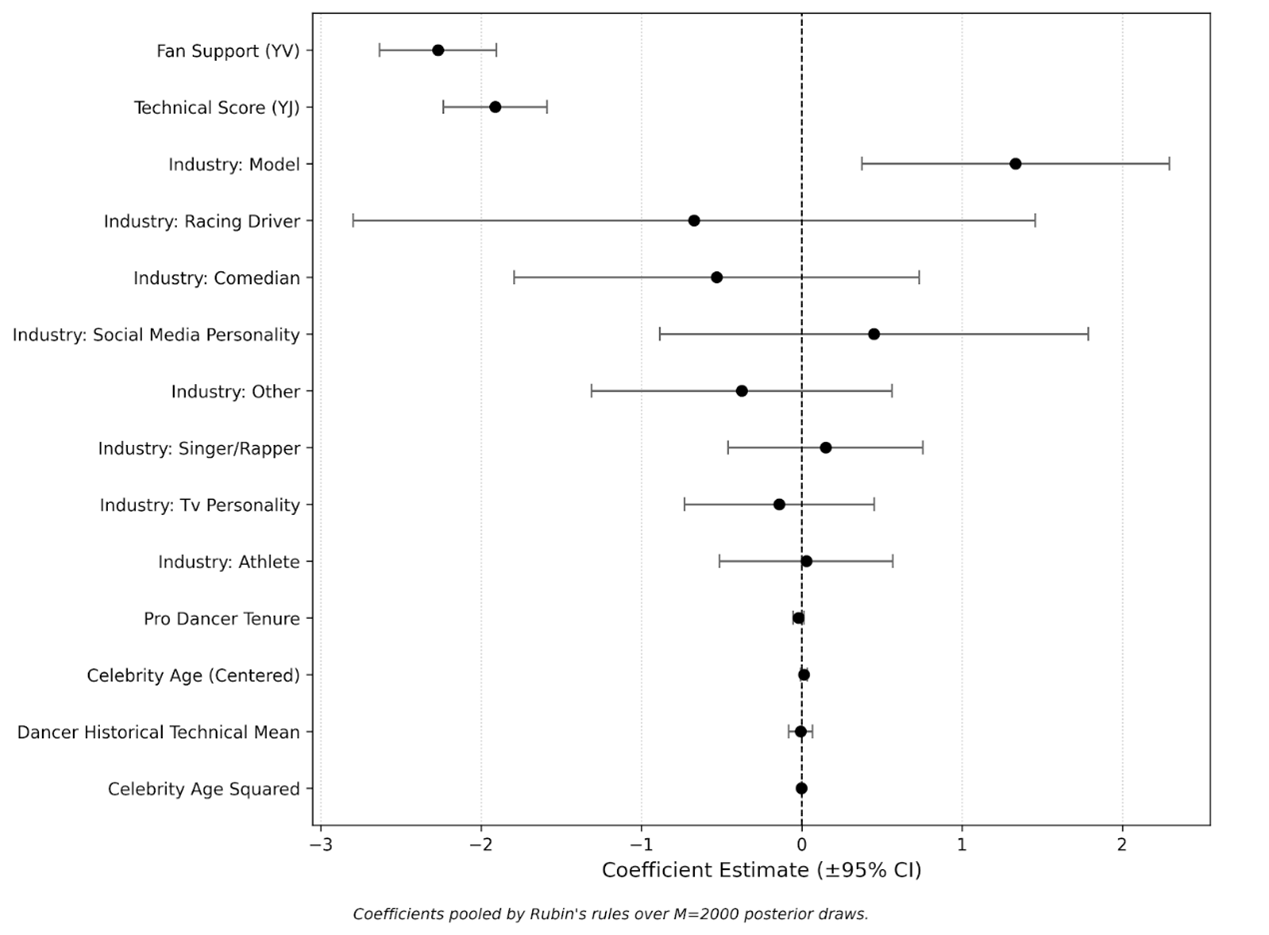
\includegraphics[width=\textwidth]{figures/Q3.3.png}
    \caption{Coefficients with 95\% intervals pooled over $M=2000$ Q1 posterior vote draws.}
    \label{fig:q3_or_forest}
  \end{subfigure}
  \hfill
  \begin{subfigure}[t]{0.53\textwidth}
    \centering
    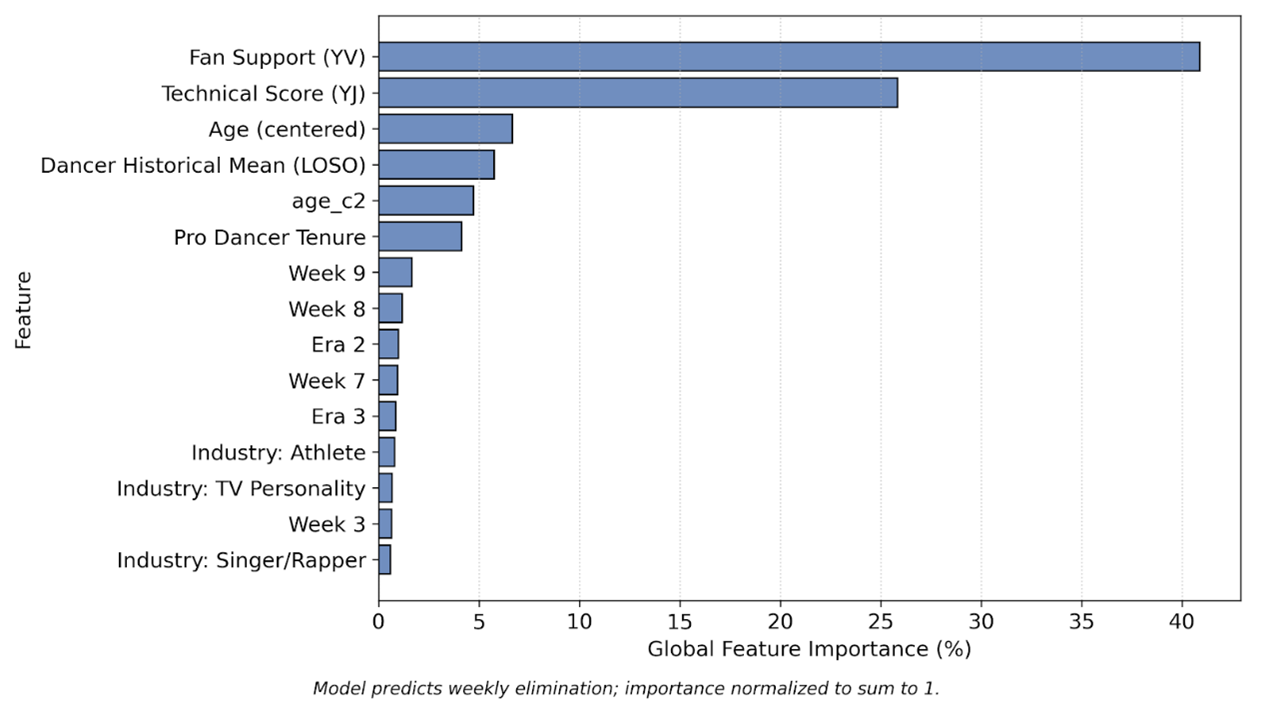
\includegraphics[width=\textwidth]{figures/Q3.4.png}
    \caption{Random forest analysis confirms the primacy of performance and fan support over secondary demographic factors.}
    \label{fig:q3_rf_importance}
  \end{subfigure}
  \caption{\textbf{Determinants of survival and robustness diagnostics.}}
  \label{fig:q3_survival_and_rf}
\end{figure}

To corroborate this driver hierarchy, we employ a nonparametric \textbf{Random Forest} diagnostic (Fig.~\ref{fig:q3_rf_importance}). The resulting importance scores confirm that elimination risk is dominated by contemporaneous performance and fan support, relegating age and professional attributes to secondary yet systematic roles\footnote{Random forests serve here solely as a robustness diagnostic .}.

Refining the functional form reveals Nonlinear Age Effects, where a quadratic specification yields a U-shaped risk profile, implying practical limits to sympathy compensation. Regarding identification, we acknowledge Matching Endogeneity due to non-random partner assignment; we therefore interpret estimates as conditional associations, utilizing Leakage-Controlled Pro Profiles to mitigate selection bias in the absence of an external instrument.









% ============================================================
% Q4: Optimization / Proposal (Replaces Problem 4)
% ============================================================
\section{The PAGS Architecture – An Optimized Elimination Mechanism  }
\label{sec:q4}

% [新增] 任务对应说明
\noindent \textit{This section addresses Task 4 by proposing the "PAGS" architecture—an optimized elimination mechanism derived from the fairness metrics established in Models II and III to reconcile meritocratic integrity with audience agency.}

\vspace{1em}

\subsection{Optimization Objectives for Meritocracy and Agency }
\label{sec:q4_analysis}

It is required to propose an alternative weekly elimination mechanism that uses only judges' scores and fan votes, and to provide evidence that the proposed mechanism should be adopted. According to the conventions established in Problems 1--3, admissible weekly inputs are restricted to: (i) the observed dynamic mean judge score $J_{i,s,t}$ (field \texttt{wt\_avg}) and its share within the week $p_{i,s,t}(J)$; and (ii) the latent fan-support simplex represented exclusively through the posterior samples $\{v^{(m)}_{s,t}\}_{m=1}^{M}$ inferred in Q1, with $M=2000$. Any substitution of $\{v^{(m)}_{s,t}\}$ by a point estimate is prohibited, because the elimination mapping can be discontinuous and the uncertainty must be propagated by construction.

The design objective is formalized as a \emph{multi-objective optimization} problem. A structural tension exists between \emph{meritocratic alignment} (technical credibility measured by the judge channel) and \emph{audience agency} (the degree to which fan votes remain outcome-determinative). The target is not a binary notion of ``fairness,'' but a \emph{tunable trade-off mechanism} whose parameters can be audited and adjusted to satisfy explicit constraints on both professionalism and agency.

\subsection{The PAGS Parametric Hybrid Framework Design }
\label{sec:q4_model}

A new elimination system, termed \textbf{PAGS (Professional--Adaptive Guard System)}, is defined as a modular architecture with three components: (A) an \emph{adaptive damping} module (the $\lambda$-mechanism) that mitigates block-voting anomalies under statistically verifiable technical collapse; (B) \emph{dynamic phased weighting} that smoothly transitions from engagement-oriented aggregation to reputation-oriented aggregation as the competition advances; and (C) a \emph{minimal-intervention guardrail} that activates only under narrowly defined violations of meritocratic alignment.

\subsubsection{Modular Definition of PAGS}
\label{sec:q4_modules}


\noindent\textbf{Module A: Adaptive Damping (the $\lambda$-Mechanism).}\phantomsection\label{sec:q4_gamma}


For each posterior sample $v^{(m)}_{s,t}$, an effective damped fan-share vector $\tilde v^{(m)}_{s,t}$ is defined by a power transform followed by simplex renormalization:
\begin{equation}
\tilde v_{i,s,t}^{(m)}(\lambda_{s,t})
=
\frac{\bigl(v_{i,s,t}^{(m)}\bigr)^{\lambda_{s,t}}}{\sum_{k\in C_{s,t}}\bigl(v_{k,s,t}^{(m)}\bigr)^{\lambda_{s,t}}},
\qquad 
\lambda_{s,t}\in[\lambda_{\min},1].
\label{eq:q4_damped_votes}
\end{equation}
When $\lambda_{s,t}=1$, the mechanism reduces to the base fan shares. When $\lambda_{s,t}<1$, head shares are compressed and tail shares are relatively elevated, thus mitigating extreme vote dominance while preserving ordinal information in typical weeks.

The damping intensity is activated exclusively by \emph{technical outliers}. Let $\bar J_{s,t}$ and $\sigma_{J,s,t}$ denote the mean and standard deviation within-weeks of $\{J_{i,s,t}:i\in C_{s,t}\}$. The technical outlier score is defined as a $z$-score
\begin{equation}
z_{i,s,t}=\frac{J_{i,s,t}-\bar J_{s,t}}{\sigma_{J,s,t}},
\qquad 
\delta_{s,t}=\max_{i\in C_{s,t}}\{0,-z_{i,s,t}\},
\label{eq:q4_zscore}
\end{equation}
and the damping coefficient is defined by a clipped linear response:
\begin{equation}
\lambda_{s,t}=\mathrm{clip}\!\left(1-\xi\cdot \min(\delta_{s,t},\delta_{\max}),\ \lambda_{\min},\ 1\right).
\label{eq:q4_gamma_def}
\end{equation}
The above formulation enforces a circuit-breaker effect only when a statistically detectable collapse in technical performance occurs, rather than during ordinary popularity fluctuations.

\medskip
\noindent\textbf{Module B: Dynamic Phased Weighting.}\phantomsection\label{sec:q4_weight}

To avoid rank-induced discontinuities, PAGS adopts a percent-style continuous composite. Let $n_{s,t}=|C_{s,t}|$ denote the number of remaining contestants in week $(s,t)$, with $n_{s,1}$ the initial cast size and $n_{\min}$ a final threshold (e.g. $n_{\min}=3$). The weight of the judge $w_{s,t}$ is defined as not decreasing as the season progresses:
\begin{equation}
w_{s,t}
=
w_{\min}
+
(w_{\max}-w_{\min})
\cdot
\frac{n_{s,1}-n_{s,t}}{n_{s,1}-n_{\min}},
\qquad 0<w_{\min}<w_{\max}<1.
\label{eq:q4_weight_schedule}
\end{equation}
This definition yields a smooth transition from participation-oriented aggregation in the early weeks to reputation-oriented aggregation in the late weeks.

\medskip
\noindent\textbf{Module C: Composite Score and Elimination Operator.}\phantomsection\label{sec:q4_score}

The observed weekly judge score $J_{i,s,t}$ is defined as the arithmetic mean over the active judging panel in week $(s,t)$:
\begin{equation}
J_{i,s,t}
=
\frac{1}{|\mathcal{G}_{i,s,t}|}\sum_{g\in \mathcal{G}_{i,s,t}} S_{i,s,t,g},
\qquad 
\mathcal{G}_{i,s,t}\subseteq \mathcal{G}_{s,t},
\quad 
N_{\mathrm{judges},s,t}=|\mathcal{G}_{s,t}|\in\{2,3,4\},
\label{eq:q4_Javg}
\end{equation}

where $S_{i,s,t,g}$ denotes the score assigned by judge $g$ and $\mathcal{G}_{i,s,t}$ collects the non-missing judges for contestant $i$ in that week. This mean-score construction stabilizes the score scale across weeks with varying panel sizes and missingness patterns.

The admissible judge share is defined via within-week simplex normalization:
\begin{equation}
p_{i,s,t}(J)=\frac{J_{i,s,t}}{\sum_{k\in C_{s,t}} J_{k,s,t}},
\qquad 
N_{\mathrm{judges},s,t}\in\{2,3,4\}.
\label{eq:q4_jshare}
\end{equation}

For each posterior draw $m$, the PAGS composite score is defined by
\begin{equation}
S_{i,s,t}^{(m)}
=
w_{s,t}\,p_{i,s,t}(J)
+
(1-w_{s,t})\,\tilde v_{i,s,t}^{(m)}(\lambda_{s,t}),
\qquad i\in C_{s,t}.
\label{eq:q4_composite}
\end{equation}
Let $m_{s,t}=|E_{s,t}|$ denote the observed number of eliminations in week $(s,t)$. The counterfactual PAGS elimination set under draw $m$ is defined as
\begin{equation}
E_{s,t}^{\mathrm{PAGS}}\!\bigl(v^{(m)}_{s,t}\bigr)
=
\mathrm{Bottom}_{m_{s,t}}
\Bigl\{
S_{i,s,t}^{(m)}: i\in C_{s,t}
\Bigr\},
\label{eq:q4_elimset}
\end{equation}
where $\mathrm{Bottom}_{m}(\cdot)$ returns the index set of the $m$ smallest entries (with deterministic tie-breaking as declared globally).

\subsubsection{The Minimal Intervention Guardrail Constraint }
\label{sec:q4_guardrail}

In reputation-sensitive late stages, a minimal guardrail is imposed to prevent the elimination of top technical performers. Define the technical top set
\begin{equation}
T_{s,t}^{K}
=
\mathrm{Top}_{K}\{p_{i,s,t}(J): i\in C_{s,t}\}.
\label{eq:q4_topk}
\end{equation}
Let $\hat E_{s,t}$ denote the baseline elimination set predicted by \eqref{eq:q4_elimset}. If $\hat E_{s,t}\cap T_{s,t}^{K}\neq\varnothing$, then each eliminated contestant in $\hat E_{s,t}\cap T_{s,t}^{K}$ is iteratively replaced by the next-lowest nonprotected contestant until $\hat E_{s,t}\cap T_{s,t}^{K}=\varnothing$. This constraint is explicitly auditable and adheres to the minimal-intervention principle: it activates only under a narrow, pre-specified violation of meritocratic alignment.

\subsection{Counterfactual Historical Simulation Evaluation }
\label{sec:q4_eval}

For each elimination week $(s,t)$, we propagate posterior draws $\{v^{(m)}_{s,t}\}_{m=1}^{M}$ through the PAGS mapping: compute $\lambda_{s,t}$ via \eqref{eq:q4_gamma_def}, obtain $\tilde v^{(m)}_{s,t}$ via \eqref{eq:q4_damped_votes}, compute $S^{(m)}_{i,s,t}$ via \eqref{eq:q4_composite}, and derive $E_{s,t}^{\mathrm{PAGS}}(v^{(m)}_{s,t})$ via \eqref{eq:q4_elimset}. Any statistic $g(\cdot)$ is estimated by Monte Carlo averaging:

\begin{equation}
\widehat g
=
\frac{1}{M}\sum_{m=1}^{M}
g\!\left(v^{(m)}_{s,t}\right),
\qquad M=2000.
\label{eq:q4_mc}
\end{equation}

We evaluate PAGS along three axes—\emph{Professionalism} ($P$), \emph{Agency} ($A$), and \emph{Drama} ($D$)—to capture distinct design objectives. Define judge-only and fan-only elimination sets:

\begin{equation}
E_{s,t}^{J}
=
\mathrm{Bottom}_{m_{s,t}}\{p_{i,s,t}(J)\},
\qquad
E_{s,t}^{F}\!\bigl(v^{(m)}_{s,t}\bigr)
=
\mathrm{Bottom}_{m_{s,t}}\{v_{i,s,t}^{(m)}\}.
\label{eq:q4_extremes}
\end{equation}
With $E_{s,t}^{\mathrm{PAGS}}(v^{(m)}_{s,t})$ given by \eqref{eq:q4_elimset}, we define
\begin{equation}
P_{s,t}
=
\frac{1}{M}\sum_{m=1}^{M}
\mathbf{1}\!\left\{
E_{s,t}^{\mathrm{PAGS}}\!\bigl(v^{(m)}_{s,t}\bigr)=E_{s,t}^{J}
\right\},
\qquad
A_{s,t}=1-P_{s,t},
\label{eq:q4_P_A}
\end{equation}
\begin{equation}
D_{s,t}
=
\frac{1}{M}\sum_{m=1}^{M}
\mathbf{1}\!\left\{
E_{s,t}^{\mathrm{PAGS}}\!\bigl(v^{(m)}_{s,t}\bigr)\neq E_{s,t}^{J}
\ \land\
E_{s,t}^{\mathrm{PAGS}}\!\bigl(v^{(m)}_{s,t}\bigr)\neq E_{s,t}^{F}\!\bigl(v^{(m)}_{s,t}\bigr)
\right\}.
\label{eq:q4_D}
\end{equation}
Cross-season summaries are stratified by historical regime to avoid conflating era effects with mechanism parameters.

Let $\theta=(w_{\min},w_{\max},\xi,\lambda_{\min},K,L)$ denote tunable parameters. We perform a finite grid search, prioritizing configurations that increase mean professionalism $\bar P$ subject to $\bar A\ge 0.5$. Table~\ref{tab:q4_pad} summarizes the resulting trade-off: compared with the percent baseline, $\bar P$ increases from $0.419$ to $0.497$, $\bar A$ remains at $0.503$, and $\bar D$ rises from $0.234$ to $0.253$, suggesting that stronger merit alignment need not mechanically reduce suspense under posterior uncertainty.


\begin{table}[t]
\centering
\caption{\textbf{Aggregate P--A--D comparison under counterfactual simulation.} Professionalism ($P$), Agency ($A$), and Drama ($D$) are averaged across elimination weeks using posterior propagation with $M=2000$.}
\label{tab:q4_pad}
\begin{tabular}{lccc}
\toprule
Mechanism & $\bar P$ & $\bar A$ & $\bar D$ \\
\midrule
Percent baseline & $0.419$ & \textbf{0.583}& $0.234$ \\
PAGS (proposed) & \textbf{0.497}& $0.503$ & \textbf{0.253}\\
\bottomrule
\end{tabular}
\end{table}

Season 27, Week 8 (Bobby Bones) represents an extreme popularity--merit divergence: the percent baseline is essentially popularity-protected, whereas PAGS activates $\lambda$-damping due to a technical outlier beyond tolerance. In contrast, Season 2, Week 3 (Jerry Rice) represents moderate underperformance.

\begin{equation}
\begin{aligned}
\widehat P_{\mathrm{elim}}^{\mathrm{pct}} &\approx 0.000 \quad &\text{(S27W8: Percent)}\\
\widehat P_{\mathrm{elim}}^{\mathrm{PAGS}} &= 0.856 \quad &\text{(S27W8: PAGS)}\\
\widehat P_{\mathrm{elim}}^{\mathrm{PAGS}} &= 0.247 \quad &\text{(S2W3: PAGS)}
\end{aligned}
\label{eq:q4_stress_probs}
\end{equation}

These contrasts indicate that damping is reserved for statistically exceptional collapse rather than routine popularity--merit tension. In summary:

\begin{quote}
\emph{PAGS does not punish popularity; it only penalizes technical incompetence that exceeds a statistical tolerance threshold.}
\end{quote}


\subsection{Managerial Implications}
\label{sec:q4_mgmt}

Two adoption-facing implications are derived from counterfactual evidence.

The Season 27 stress test shows that the percent baseline yields $\widehat P_{\mathrm{elim}}^{\mathrm{pct}}\approx 0$, whereas PAGS yields $\widehat P_{\mathrm{elim}}^{\mathrm{PAGS}}=0.856$, mitigating reputation-damaging outcomes without discretionary producer intervention.

Agency remains $\bar A=0.503$, indicating that audience votes retain a quantifiable lever. Meanwhile, $\bar D$ increases ($0.234\rightarrow 0.253$), implying that the proposed system does not collapse into a single-channel deterministic process. Together, these properties support adoption when engagement and technical credibility are jointly prioritized.


\subsection{Boundary Analysis and Causal Limitations }
\label{sec:q4_limits}

All comparisons are conditional counterfactual simulations under fixed historical data and inferred fan support; no causal claim is made regarding ratings, long-run fairness, or behavioral adaptation under deployment.

Because $\mathbf v_{s,t}$ is unobserved, all reported quantities are functionals of $\{v^{(m)}_{s,t}\}$. While $M=2000$ supports uncertainty propagation, weeks with diffuse posteriors can yield wider uncertainty bands in mechanism comparisons.

The judge share $p_{i,s,t}(J)$ is computed from the weekly mean score $J_{i,s,t}$. Smaller panels increase the sampling variability of $J_{i,s,t}$ and hence $p_{i,s,t}(J)$, so a fixed $w_{s,t}$ may be mildly miscalibrated in small-panel weeks (notably Season 34 with $N_{\mathrm{judges},s,t}=2$). No explicit variance correction is imposed; in deployment, robustness can be audited by perturbing $w_{s,t}$ at a scale proportional to $N_{\mathrm{judges},s,t}^{-1/2}$.

Historical eliminations arise under heterogeneous regimes (Rank/Percent/Judges’ Save); accordingly, interpretation is restricted to regime-aware reporting, and cross-era aggregation is descriptive rather than causal.

Although the parameterization is low-dimensional and selected on a finite grid, estimates can be influenced by a small number of extreme weeks. Recommended audits include reporting the trigger frequency of $\lambda$-damping, the frequency of guardrail replacements, and robustness to perturbations of extreme fan-share scenarios.

















% =========================================================
% Section 7 (Final Trim): Sensitivity & Robustness (O-Award audit style)
% Target length: ~1.0–1.5 pages (single-column MCM template)
% =========================================================

\section{Sensitivity Analysis and Model Robustness Checks}
\label{sec:robustness}

\textbf{Audit objective.}
All Q2--Q4 claims are \emph{posterior-averaged} functionals propagated from Q1 (Monte Carlo, $M=2000$). We therefore audit robustness along three axes: \textbf{(i) statistical stability + Bayesian prior defense} (Q1--Q2), \textbf{(ii) structural invariance to model class} (Q3), and \textbf{(iii) mechanism resilience with a stability region (not ``magic numbers'')} (Q4), plus explicit safe-operation constraints.

\vspace{-0.35em}
\subsection{Statistical stability \& prior defense (Q1--Q2)}
\vspace{-0.35em}

Define the prefix-to-full convergence diagnostic
\begin{equation}
\Delta_{L1}(M')=\left\|\bar v_{M'}-\bar v_{2000}\right\|_1,
\label{eq:l1def}
\end{equation}
where $\bar v_{M'}$ is the posterior mean fan-share vector computed from the first $M'$ draws. On the audited corner week (S27W8), $\Delta_{L1}(800)=2.225\times10^{-3}$ and $\Delta_{L1}(1500)=1.323\times10^{-3}$ (Fig.~\ref{fig:robust_panels}a), indicating that $M=2000$ lies in the plateau regime and downstream summaries are not driven by finite-sample Monte Carlo error.
The posterior is constraint-dominated:
\[
p(v_{s,t}\mid\cdot)\ \propto\ \pi_{\beta}(v_{s,t})\cdot \mathbf{1}\{v_{s,t}\in\mathcal{A}_{s,t}\},
\]
so feasibility $\mathcal{A}_{s,t}$ shapes posterior mass more strongly than the Dirichlet curvature. On S27W8, a prior sweep over $\beta\in\{0,0.5,1,2,5\}$ (Base=$\beta=0$ uniform) yields stable summaries: the posterior mean shifts only $0.2027\to0.1997$ ($\approx$1.5\%), the CI width remains within 0.0670--0.0685, and the anomaly rank remains 1 (Table~\ref{tab:prior_sens_short}), addressing the prior-sensitivity concern.

Rule comparisons are computed over the full posterior ensemble. Rank vs.\ Percent differs non-trivially ($P_{\mathrm{diff}}=0.260$, $D_{\exp}=0.485$), and in the Agency regime Percent improves alignment and global consistency ($FAI_{\mathrm{Pct}}=0.277$, $\rho_{\mathrm{Pct}}=0.765$); thus the conclusion is supported at the distribution level rather than by posterior means alone.


\vspace{1ex}


\vspace{-0.45em}
\begin{table}[H]
\centering
\caption{Prior sensitivity audit (Q1, S27W8; Base=$\beta=0$ uniform). The anomaly signal is stable across a wide prior grid, indicating constraint-dominated inference.}
\label{tab:prior_sens_short}
\scriptsize
\setlength{\tabcolsep}{15.3pt}  
\renewcommand{\arraystretch}{0.93}
\begin{tabular}{@{}cccccc@{}}
\toprule
$\beta$ & Accept & Mean & 95\% CI & Rank & $L_1$ vs.\ Base \\
\midrule
0.0 & 0.2098 & 0.2027 & [0.1744,0.2414] & 1 & 0.0000 \\
0.5 & 0.2227 & 0.2026 & [0.1741,0.2414] & 1 & 0.0027 \\
1.0 & 0.2345 & 0.2023 & [0.1739,0.2411] & 1 & 0.0062 \\
2.0 & 0.2610 & 0.2015 & [0.1731,0.2415] & 1 & 0.0130 \\
5.0 & 0.3266 & 0.1997 & [0.1703,0.2388] & 1 & 0.0350 \\
\bottomrule
\end{tabular}
\vspace{-1.0em}
\end{table}

\vspace{-0.25em}
\subsection{Methodological invariance (Q3)}
\vspace{-0.35em}

\noindent ``Dual-Protection'' survives a change of hypothesis class: a parametric discrete-time hazard model and a non-parametric Random Forest both prioritize \emph{fan support} ($YV$) and \emph{technical score} ($YJ$) as dominant protective drivers. Quantitatively, among shared substantive covariates $\{YV,YJ,\mathrm{age}_c,\mathrm{age}_c^2,\mathrm{tenure},\mu_J\}$, the rank agreement between hazard effect magnitudes and RF importances is $\rho_S=0.657$ (Spearman), supporting \textbf{driver hierarchy invariance} rather than functional-form dependence.

\vspace{-0.15em}
\subsection{Mechanism resilience \& stability region (Q4)}
\vspace{-0.35em}

Bobby Bones serves as an extreme-value validation: under the Percent baseline the case is effectively popularity-protected, whereas PAGS activates the safeguard and yields $p_{\mathrm{elim}}^{\mathrm{PAGS}}=0.856$, indicating correction under reputational-risk extremes.

Across perturbations, $\gamma$ primarily governs activation frequency without inducing systematic distortion: $\rho_S(\gamma,D)=-0.056$ ($p=0.362$), while $\rho_S(\gamma,\mathbf{1}_{\text{guardrail}})=0.186$ ($p=0.0024$). Activation is $0$ for $\gamma\le0.95$ (n=24) and $0.292$ for $\gamma>0.95$ (n=240), suggesting an empirical transition; Fig.~\ref{fig:robust_panels}b delineates a contiguous region over $(\gamma,w)$ in which activation is tunable and distortion remains bounded, mitigating concerns of ad hoc threshold dependence.

The safe-operation logic is summarized by three flagged conditions. Low-variance judge weeks warrant disabling z-score triggering and reverting to standard Percent to avoid hypersensitive activation. Save-era weeks motivate restricting PAGS to within-tier correction rather than claiming full-field reordering. Weak identifiability (unusually low acceptance or wide posteriors) warrants an audit-only flag and avoidance of high-stakes intervention.

Collectively, these audits support that Percent (agency), Dual-Protection (driver hierarchy), and PAGS (tail-risk safeguard) remain robust and interpretable under the stated constraints.


% -------------------------
% Two compact figure placeholders side-by-side (space-efficient)
% -------------------------
\vspace{-0.55em}
\begin{figure}[H]
\centering
\begin{minipage}{0.5\linewidth}
  \centering
  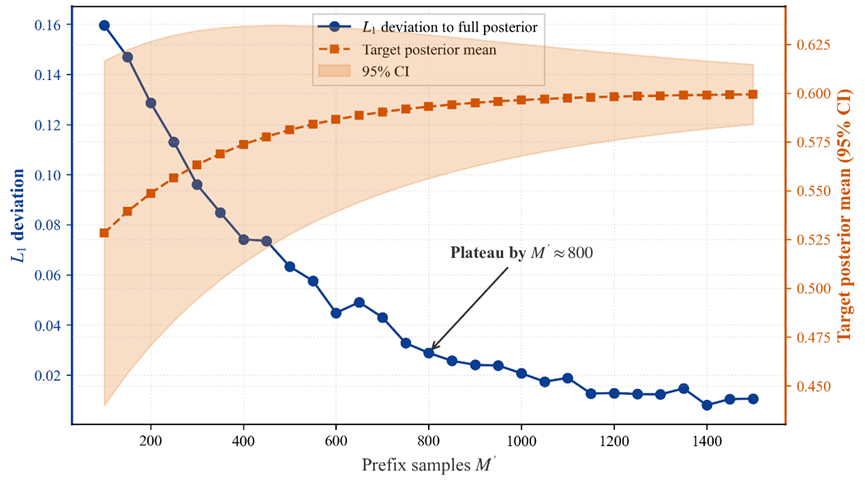
\includegraphics[width=0.95\linewidth]{figures/S1.png}
\end{minipage}\hfill
\begin{minipage}{0.5\linewidth}
  \centering
  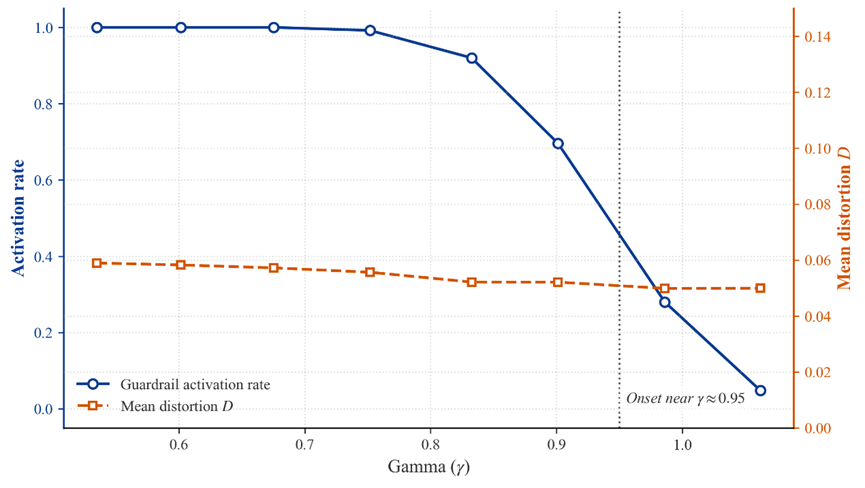
\includegraphics[width=0.95\linewidth]{figures/S2.png}
\end{minipage}
\caption{Compact robustness visuals for rapid audit.}
\label{fig:robust_panels}
\vspace{-1.0em}
\end{figure}




% ============================================================
% Model Evaluation: Strengths and Weaknesses (Concise Version)
% ============================================================
\section{Strengths and Limitations}
\label{sec:evaluation}

% ============================================================
% Model Evaluation: Strengths and Weaknesses (Compressed Layout)
% ============================================================



% 开启小字号模式，并缩减段后间距
\begingroup

\setlength{\parskip}{0pt} 

We assess the validity of our framework by evaluating its operational identifiability, structural consistency, and interpretability under partial observability.

%\vspace{-0.8em} % 强制缩减标题与列表的距离
\noindent\textbf{Strengths.}
\begin{enumerate}
    % 强制压缩列表内部间距
    \setlength{\itemsep}{0pt}
    \setlength{\parskip}{0pt}
    \setlength{\parsep}{0pt}
    
    \item \textbf{Unified Uncertainty Propagation.} 
    By propagating the full posterior distribution ($M=2000$ draws) rather than point estimates, our framework ensures operational identifiability and avoids the false precision of deterministic models ($\mathrm{PPC} \approx 0.905$).

    %\item \textbf{Structural Isolation via Counterfactuals.} 
    %Our within-week design isolates the aggregation rule as the sole independent variable, confirming that observed outcome divergences are inherent systemic properties rather than random anomalies.

    \item \textbf{Robust Dual-Signal Attribution.} 
    The hazard model effectively decouples meritocratic (judge) from democratic (fan) signals, with parametric findings validated by the consistent feature rankings of nonparametric random forests.

    \item \textbf{Stress-Tested Mechanism Design.} 
    The proposed PAGS architecture is validated against historical "worst-case" controversies, demonstrating quantifiable fairness improvements without sacrificing commercial audience agency.
\end{enumerate}

%\vspace{-0.8em} % 强制缩减段落间距
\noindent\textbf{Limitations.}
\begin{enumerate}
    % 强制压缩列表内部间距
    \setlength{\itemsep}{0pt}
    \setlength{\parskip}{0pt}
    \setlength{\parsep}{0pt}

    \item \textbf{Dependence on Latent Inference.} 
    All findings remain conditional on the inverse reconstruction; weeks with sparse data or weak correlations yield diffuse posteriors that inherently widen downstream uncertainty bands.

    \item \textbf{Static Behavioral Assumption.} 
    The counterfactuals assume a \textit{ceteris paribus} environment, isolating mechanical effects while neglecting potential long-term game-theoretic adaptations by judges or contestants.

    \item \textbf{Parametric Sensitivity.} 
    The proposed system relies on tuned damping parameters, which require continuous auditing to ensure robustness against rare, extreme voting distributions in future seasons.
\end{enumerate}
\vspace{1ex}
\noindent\textbf{Conclusion.}  

Overall, this work establishes an uncertainty-aware audit framework for DWTS-style hybrid decision rules under unobserved voting. With regime-consistent vote reconstruction (PPC $=90.5\%$), quantified rule-induced volatility ($26\%$ of historical weeks), and cross-model driver-invariance evidence, we provide a systematic diagnostic of the conditions and origins of legitimacy risks. PAGS maintains a near-neutral performance baseline ($P \approx 0.5$) to preserve audience agency while enforcing a transparent circuit-breaker that corrects extreme popularity--merit divergences (e.g., the Bobby Bones corner case), and the producer-facing memo translates these audit findings into deployable guidance.


\endgroup

\newpage
% ============================================================
% 6.memo.tex  (Embedded Memorandum for MCM/ICM 2026 Problem C)
% Usage in main.tex: \clearpage % ============================================================
% 6.memo.tex  (Embedded Memorandum for MCM/ICM 2026 Problem C)
% Usage in main.tex: \clearpage % ============================================================
% 6.memo.tex  (Embedded Memorandum for MCM/ICM 2026 Problem C)
% Usage in main.tex: \clearpage \input{6.memo.tex} \clearpage
% NOTE: This file contains NO preamble and NO \documentclass.
% ============================================================

% --------- page break + optional page style ----------

\thispagestyle{empty} % 如你希望保留页眉页脚，可删掉这一行
\setlength{\fboxsep}{6pt}
\noindent\fbox{%
\begin{minipage}{0.97\textwidth}
\begingroup
\footnotesize


% --------- Title ----------
\vspace{1em} % ↑ 增大标题到边框上边距（可调：0.4em~1.0em）
\begin{center}
    {\Large\bfseries MEMORANDUM}
\end{center}
\vspace{-1.7em} % ↓ 减小标题下方间距（可调：-0.2em~-0.6em）


\vspace{0.3em}
\noindent\rule{\textwidth}{0.4pt}
\vspace{0.6em}

% --------- Header block (To/From/Date/Subject + optional CC/Attachments) ----------
% 只用 tabular（不依赖 tabularx），确保最大兼容性
\noindent\begin{tabular}{@{}p{0.14\textwidth}p{0.84\textwidth}@{}}

\textbf{To:}      & Producers, \textit{Dancing with the Stars} (DWTS) \\[0.25em]

\textbf{From:}    & MCM/ICM 2026 Team \#\underline{2619541} (Problem C) \\[0.25em]

\textbf{Date:}    & 2 February 2026 \\[0.25em]

\textbf{Subject:} & Impact of Combining Judge Scores and Fan Votes: Evidence and Recommendations Based on Q1--Q4 \\[0.25em]

%\textbf{CC:}      & Executive Producer / Voting Operations Partner / Rules \& Compliance Lead (optional) \\[0.25em]
\textbf{Attach:}  &  A. One-page rule comparison; B. Parameter notes; C. Case review of controversial weeks
\end{tabular}

\vspace{0.6em}
\noindent\rule{\textwidth}{0.4pt}
\vspace{0.8em}

% ============================================================
% Body (Memo should be non-technical but evidence-backed)
% ============================================================

\noindent\textbf{Purpose.}
This memorandum summarizes how alternative vote-combination rules change DWTS outcomes and recommends a transparent system that balances competitive credibility and audience agency.

\vspace{0.4em}

\noindent\textbf{Evidence base (Q1--Q4).}
Because fan vote counts are unobserved, we infer rule-consistent fan vote shares (Q1), run week-level counterfactual comparisons across Rank/Percent and save variants (Q2–Q3), and test an interpretable monotone safeguard against extreme vote concentration (Q4).

\vspace{0.4em}

\noindent\textbf{Key findings.}
\begin{itemize}
    \item \textbf{Aggregation choice meaningfully changes eliminations.}
    Switching between rank-based aggregation and percent-based aggregation changes the eliminated contestant in abou \textbf{26\%} of elimination weeks.

    \item \textbf{Percent-based aggregation better reflects overall audience ordering.}
    Percent-based aggregation better matches the fan-support ordering (\textbf{0.765} vs \textbf{0.678} average rank-correlation).

    \item \textbf{Both channels matter; over-correcting either direction creates risk.}
    Both judge performance and fan support materially affect elimination risk; extreme tilts toward either channel increase fairness and credibility concerns.

    \item \textbf{Judges’ Save is best treated as an exception-handling tool, not a substitute for transparent rules.}
    A Save mechanism can protect strong technical performers when short-term voting fluctuations place them at risk, but discretionary intervention can also increase perceived unfairness if criteria are not explicit and stable.
\end{itemize}

\vspace{0.4em}

\noindent\textbf{Recommendations for future seasons.}
\begin{enumerate}
    \item \textbf{Use Percent-based aggregation as the default backbone.}
    It more directly translates audience support into outcomes and is easier to explain to viewers, reducing “black-box” perceptions.

    \item \textbf{Add a pre-announced safeguard against extreme vote-lock-in.}
    When fan votes become unusually concentrated, apply a monotone compression that \emph{preserves ordering} but reduces excessive margins. This mitigates cases where performance becomes effectively irrelevant due to outsized vote blocs.

    \item \textbf{Adopt stage-dependent weighting to reflect season goals.}
    Use relatively higher audience influence early to encourage engagement, and gradually increase the role of technical judging later to strengthen the credibility of finalists and the champion.

    \item \textbf{If keeping Judges’ Save, constrain and standardize it.}
    Limit its scope (e.g., only within Bottom-2), specify when it can be used (e.g., mid-to-late season), and tie it to transparent performance-based criteria. This preserves its “professional safeguard” function while reducing perceived arbitrariness.
\end{enumerate}

\vspace{0.4em}

\noindent\textbf{Action requested.}
We recommend deciding and announcing before the season begins: (1) Percent backbone, (2) safeguard trigger/strength parameters, and (3) whether Judges’ Save is used and, if so, its constraints and criteria.

\vspace{0.4em}

\noindent\textbf{Bottom line.}
A Percent backbone with a published safeguard and stage-dependent weights preserves engagement while reducing extreme outcomes; any Judges’ Save should be strictly rule-bound.

\endgroup
\end{minipage}}

% --------- end of memo ----------
 \clearpage
% NOTE: This file contains NO preamble and NO \documentclass.
% ============================================================

% --------- page break + optional page style ----------

\thispagestyle{empty} % 如你希望保留页眉页脚，可删掉这一行
\setlength{\fboxsep}{6pt}
\noindent\fbox{%
\begin{minipage}{0.97\textwidth}
\begingroup
\footnotesize


% --------- Title ----------
\vspace{1em} % ↑ 增大标题到边框上边距（可调：0.4em~1.0em）
\begin{center}
    {\Large\bfseries MEMORANDUM}
\end{center}
\vspace{-1.7em} % ↓ 减小标题下方间距（可调：-0.2em~-0.6em）


\vspace{0.3em}
\noindent\rule{\textwidth}{0.4pt}
\vspace{0.6em}

% --------- Header block (To/From/Date/Subject + optional CC/Attachments) ----------
% 只用 tabular（不依赖 tabularx），确保最大兼容性
\noindent\begin{tabular}{@{}p{0.14\textwidth}p{0.84\textwidth}@{}}

\textbf{To:}      & Producers, \textit{Dancing with the Stars} (DWTS) \\[0.25em]

\textbf{From:}    & MCM/ICM 2026 Team \#\underline{2619541} (Problem C) \\[0.25em]

\textbf{Date:}    & 2 February 2026 \\[0.25em]

\textbf{Subject:} & Impact of Combining Judge Scores and Fan Votes: Evidence and Recommendations Based on Q1--Q4 \\[0.25em]

%\textbf{CC:}      & Executive Producer / Voting Operations Partner / Rules \& Compliance Lead (optional) \\[0.25em]
\textbf{Attach:}  &  A. One-page rule comparison; B. Parameter notes; C. Case review of controversial weeks
\end{tabular}

\vspace{0.6em}
\noindent\rule{\textwidth}{0.4pt}
\vspace{0.8em}

% ============================================================
% Body (Memo should be non-technical but evidence-backed)
% ============================================================

\noindent\textbf{Purpose.}
This memorandum summarizes how alternative vote-combination rules change DWTS outcomes and recommends a transparent system that balances competitive credibility and audience agency.

\vspace{0.4em}

\noindent\textbf{Evidence base (Q1--Q4).}
Because fan vote counts are unobserved, we infer rule-consistent fan vote shares (Q1), run week-level counterfactual comparisons across Rank/Percent and save variants (Q2–Q3), and test an interpretable monotone safeguard against extreme vote concentration (Q4).

\vspace{0.4em}

\noindent\textbf{Key findings.}
\begin{itemize}
    \item \textbf{Aggregation choice meaningfully changes eliminations.}
    Switching between rank-based aggregation and percent-based aggregation changes the eliminated contestant in abou \textbf{26\%} of elimination weeks.

    \item \textbf{Percent-based aggregation better reflects overall audience ordering.}
    Percent-based aggregation better matches the fan-support ordering (\textbf{0.765} vs \textbf{0.678} average rank-correlation).

    \item \textbf{Both channels matter; over-correcting either direction creates risk.}
    Both judge performance and fan support materially affect elimination risk; extreme tilts toward either channel increase fairness and credibility concerns.

    \item \textbf{Judges’ Save is best treated as an exception-handling tool, not a substitute for transparent rules.}
    A Save mechanism can protect strong technical performers when short-term voting fluctuations place them at risk, but discretionary intervention can also increase perceived unfairness if criteria are not explicit and stable.
\end{itemize}

\vspace{0.4em}

\noindent\textbf{Recommendations for future seasons.}
\begin{enumerate}
    \item \textbf{Use Percent-based aggregation as the default backbone.}
    It more directly translates audience support into outcomes and is easier to explain to viewers, reducing “black-box” perceptions.

    \item \textbf{Add a pre-announced safeguard against extreme vote-lock-in.}
    When fan votes become unusually concentrated, apply a monotone compression that \emph{preserves ordering} but reduces excessive margins. This mitigates cases where performance becomes effectively irrelevant due to outsized vote blocs.

    \item \textbf{Adopt stage-dependent weighting to reflect season goals.}
    Use relatively higher audience influence early to encourage engagement, and gradually increase the role of technical judging later to strengthen the credibility of finalists and the champion.

    \item \textbf{If keeping Judges’ Save, constrain and standardize it.}
    Limit its scope (e.g., only within Bottom-2), specify when it can be used (e.g., mid-to-late season), and tie it to transparent performance-based criteria. This preserves its “professional safeguard” function while reducing perceived arbitrariness.
\end{enumerate}

\vspace{0.4em}

\noindent\textbf{Action requested.}
We recommend deciding and announcing before the season begins: (1) Percent backbone, (2) safeguard trigger/strength parameters, and (3) whether Judges’ Save is used and, if so, its constraints and criteria.

\vspace{0.4em}

\noindent\textbf{Bottom line.}
A Percent backbone with a published safeguard and stage-dependent weights preserves engagement while reducing extreme outcomes; any Judges’ Save should be strictly rule-bound.

\endgroup
\end{minipage}}

% --------- end of memo ----------
 \clearpage
% NOTE: This file contains NO preamble and NO \documentclass.
% ============================================================

% --------- page break + optional page style ----------

\thispagestyle{empty} % 如你希望保留页眉页脚，可删掉这一行
\setlength{\fboxsep}{6pt}
\noindent\fbox{%
\begin{minipage}{0.97\textwidth}
\begingroup
\footnotesize


% --------- Title ----------
\vspace{1em} % ↑ 增大标题到边框上边距（可调：0.4em~1.0em）
\begin{center}
    {\Large\bfseries MEMORANDUM}
\end{center}
\vspace{-1.7em} % ↓ 减小标题下方间距（可调：-0.2em~-0.6em）


\vspace{0.3em}
\noindent\rule{\textwidth}{0.4pt}
\vspace{0.6em}

% --------- Header block (To/From/Date/Subject + optional CC/Attachments) ----------
% 只用 tabular（不依赖 tabularx），确保最大兼容性
\noindent\begin{tabular}{@{}p{0.14\textwidth}p{0.84\textwidth}@{}}

\textbf{To:}      & Producers, \textit{Dancing with the Stars} (DWTS) \\[0.25em]

\textbf{From:}    & MCM/ICM 2026 Team \#\underline{2619541} (Problem C) \\[0.25em]

\textbf{Date:}    & 2 February 2026 \\[0.25em]

\textbf{Subject:} & Impact of Combining Judge Scores and Fan Votes: Evidence and Recommendations Based on Q1--Q4 \\[0.25em]

%\textbf{CC:}      & Executive Producer / Voting Operations Partner / Rules \& Compliance Lead (optional) \\[0.25em]
\textbf{Attach:}  &  A. One-page rule comparison; B. Parameter notes; C. Case review of controversial weeks
\end{tabular}

\vspace{0.6em}
\noindent\rule{\textwidth}{0.4pt}
\vspace{0.8em}

% ============================================================
% Body (Memo should be non-technical but evidence-backed)
% ============================================================

\noindent\textbf{Purpose.}
This memorandum summarizes how alternative vote-combination rules change DWTS outcomes and recommends a transparent system that balances competitive credibility and audience agency.

\vspace{0.4em}

\noindent\textbf{Evidence base (Q1--Q4).}
Because fan vote counts are unobserved, we infer rule-consistent fan vote shares (Q1), run week-level counterfactual comparisons across Rank/Percent and save variants (Q2–Q3), and test an interpretable monotone safeguard against extreme vote concentration (Q4).

\vspace{0.4em}

\noindent\textbf{Key findings.}
\begin{itemize}
    \item \textbf{Aggregation choice meaningfully changes eliminations.}
    Switching between rank-based aggregation and percent-based aggregation changes the eliminated contestant in abou \textbf{26\%} of elimination weeks.

    \item \textbf{Percent-based aggregation better reflects overall audience ordering.}
    Percent-based aggregation better matches the fan-support ordering (\textbf{0.765} vs \textbf{0.678} average rank-correlation).

    \item \textbf{Both channels matter; over-correcting either direction creates risk.}
    Both judge performance and fan support materially affect elimination risk; extreme tilts toward either channel increase fairness and credibility concerns.

    \item \textbf{Judges’ Save is best treated as an exception-handling tool, not a substitute for transparent rules.}
    A Save mechanism can protect strong technical performers when short-term voting fluctuations place them at risk, but discretionary intervention can also increase perceived unfairness if criteria are not explicit and stable.
\end{itemize}

\vspace{0.4em}

\noindent\textbf{Recommendations for future seasons.}
\begin{enumerate}
    \item \textbf{Use Percent-based aggregation as the default backbone.}
    It more directly translates audience support into outcomes and is easier to explain to viewers, reducing “black-box” perceptions.

    \item \textbf{Add a pre-announced safeguard against extreme vote-lock-in.}
    When fan votes become unusually concentrated, apply a monotone compression that \emph{preserves ordering} but reduces excessive margins. This mitigates cases where performance becomes effectively irrelevant due to outsized vote blocs.

    \item \textbf{Adopt stage-dependent weighting to reflect season goals.}
    Use relatively higher audience influence early to encourage engagement, and gradually increase the role of technical judging later to strengthen the credibility of finalists and the champion.

    \item \textbf{If keeping Judges’ Save, constrain and standardize it.}
    Limit its scope (e.g., only within Bottom-2), specify when it can be used (e.g., mid-to-late season), and tie it to transparent performance-based criteria. This preserves its “professional safeguard” function while reducing perceived arbitrariness.
\end{enumerate}

\vspace{0.4em}

\noindent\textbf{Action requested.}
We recommend deciding and announcing before the season begins: (1) Percent backbone, (2) safeguard trigger/strength parameters, and (3) whether Judges’ Save is used and, if so, its constraints and criteria.

\vspace{0.4em}

\noindent\textbf{Bottom line.}
A Percent backbone with a published safeguard and stage-dependent weights preserves engagement while reducing extreme outcomes; any Judges’ Save should be strictly rule-bound.

\endgroup
\end{minipage}}

% --------- end of memo ----------




\clearpage
\newpage

% =========================
% References (integrated)
% =========================
\begin{thebibliography}{99}

\bibitem{Saari D G}
Saari D G. Disposing dictators, demystifying voting paradoxes[J]. Mathematical and Computer Modelling, 2008, 48(9-10): 1671-1673 

\bibitem{Little R J A}
Little R J A, Rubin D B. Statistical analysis with missing data[M]. John Wiley \& Sons, 2019. 

\bibitem{Pawlowsky-Glahn V}
Pawlowsky-Glahn V, Egozcue J J, Tolosana-Delgado R. Modeling and analysis of compositional data[M]. John Wiley \& Sons, 2015. 

\bibitem{Egozcue J J}
Egozcue J J, Pawlowsky-Glahn V, Mateu-Figueras G, et al. Isometric logratio transformations for compositional data analysis[J]. Mathematical geology, 2003, 35(3): 279-300. 

\bibitem{Allison P D.}
Allison P D. Discrete-time methods for the analysis of event histories[J]. Sociological methodology, 1982, 13: 61-98. 

\bibitem{Ginsburgh V}
Ginsburgh V, Noury A G. The Eurovision song contest. Is voting political or cultural?[J]. European Journal of Political Economy, 2008, 24(1): 41-52. 

\bibitem{Saari D G}
Saari D G. Basic geometry of voting[M]. Springer Science \& Business Media, 1995. 

\bibitem{Gemser G}
Gemser G, Van Oostrum M, Leenders M A A M. The impact of film reviews on the box office performance of art house versus mainstream motion pictures[J]. Journal of Cultural Economics, 2007, 31(1): 43-63. 



\end{thebibliography}


%\clearpage
%\appendix
\section{Appendices}
\label{app:supp}



\newpage
\AImatter
\begin{ReportAiUse}{9}



\bibitem{AI1}
YouDaoFanyi, YouDao Translate（（Feb 2,2026 version）


Help us translate this question into Chinese, and also translate some parts of our paper into English.






\bibitem{AI2}

Google Gemini (（Feb 2,2026 version, Gemini1.5 pro)

Query1:Color scheme optimization: Request the AI to recommend color schemes that comply with academic standards for the existing matplotlib charts (bar charts, box plots, flowcharts) (such as dark blue/light gray, blue/orange complementary colors, transparent blue/grey, etc.), with distinct visual hierarchy to highlight the core data (PAGS model).


Output:    Gemini has recommended some suitable color schemes for us to choose from, such as blue-white combination and blue-orange combination.





\bibitem{AI3}

OpenAI ChatGPT (Feb 2, 2026 version, ChatGPT-4 )


Query1: \\Help us search for relevant literature on the competition topics in recent years to provide inspiration.


Output:   GPT has generated relevant papers related to the competition topic for our reference. All the papers we used have been included in the references.




\bibitem{AI4}

OpenAI ChatGPT (Feb 2, 2026 version, ChatGPT-4 )


Query1: Provide suggestions for adjusting the LaTeX code to make the layout of the paper more aesthetically pleasing.


Output:  GPT provided suggestions for adjusting the LaTeX code, including aspects such as line spacing, distribution of first-level and second-level headings, etc.   









\end{ReportAiUse}




\end{document}

